\documentclass[12pt]{article}
\usepackage[margin=1in]{geometry} 
\usepackage{amsmath,amsthm,amssymb,amsfonts}
\usepackage{enumitem}
\usepackage{tabu}
\usepackage{xcolor}
\usepackage{mathtools}
\usepackage{tcolorbox} 
\usepackage{changepage} 
\usepackage{kpfonts}
\usepackage{picture}
\usepackage{venndiagram}
\usepackage{pgfplots}
\usepackage{pgfplotstable}
\usepackage{tikz}
\usepackage{tkz-euclide}

\tikzset{
  open/.style = {circle, minimum size=2mm,draw, fill=white,inner sep=0pt},
  closed/.style = {circle, minimum size=2mm, fill, inner sep=0pt},
}

% arrow and line for 'tkzPointShowCoord'
\makeatletter
\tikzset{arrow coord style/.style={%
    densely dashed,
    \tkz@euc@linecolor,
    %>=stealth',
    %->,
    }}
    \tikzset{xcoord style/.style={%
    \tkz@euc@labelcolor,
    font=\normalsize,text height=1ex,
    inner sep = 0pt,
    outer sep = 0pt,
    fill=\tkz@fillcolor,
    below=6pt
    }} 
\tikzset{ycoord style/.style={%
    \tkz@euc@labelcolor,
    font=\normalsize,text height=1ex, 
    inner sep = 0pt,
    outer sep = 0pt, 
    fill=\tkz@fillcolor,
    left=6pt
    }}  
\makeatother

\newcommand{\N}{\mathbb{N}}
\newcommand{\Z}{\mathbb{Z}}
\newcommand{\R}{\mathbb{R}}
\newcommand{\faps}{(\Omega, \field, \mathbb{P})}

\newcommand{\field}{\mathcal{F}}
\newcommand{\prob}[1]{\mathbb{P}(#1)}
\newcommand{\condprob}[2]{\mathbb{P}(#1 \text{ } \lvert \text{ } #2)}
\newcommand{\probtext}[1]{\mathbb{P}(\text{#1})}

\newcommand\gauss[2]{1/(#2*sqrt(2*pi))*exp(-((x-#1)^2)/(2*#2^2))} 
% Gauss function, parameters mu and sigma

\renewcommand\labelitemi{---}

\newcommand{\nspace}{\vspace*{.5cm}}
\newcommand{\nline}{\nspace \noindent}

\newcommand{\expected}[1]{\text{E}(#1)}
\newcommand{\variance}[1]{\text{V}(#1)}

\newenvironment{nscenter}
 {\parskip=0pt\par\nopagebreak\centering}
 {\par\noindent\ignorespacesafterend}
 
\def\SPSB#1#2{\rlap{\textsuperscript{\textcolor{black}{#1}}}\SB{#2}}
 
\begin{document}
\title{%
  MATH 487: Probability Theory \\
  \large University of Nebraska-Lincoln, Fall 2017}
\author{Jacob Shiohira}
\maketitle

\vspace*{3cm}

\noindent
The textbook used for this class is \textbf{asdf} by .

\newpage

% ================================================================================================================================
% ================================================================================================================================
\section*{CHAPTER 1: PRELIMINARIES}
% ================================================================================================================================
% ================================================================================================================================

% ==================================================
\begin{flushright}
\textbf{Date:} $8/22$ 
\end{flushright}
% ==================================================

\noindent
The sample space $\Omega$ is the set of all outcomes of an experiment. For a few examples, we'll consider different types of sample spaces using descriptors such as finite, infinite, countable, and uncountable.

\vspace{.3cm}
\subsection*{Finite and Countable}
\begin{tcolorbox}
\textbf{Example:} Toss a coin twice - "$H$" for heads and "$T$" for tails,

\begin{equation*}
\Omega = \big \{ (H,H), (H,T), (T,H), (T,T) \big \}
\end{equation*}

\noindent
The cardinality of $\Omega$ is then $|\Omega|=4$. The sample space for this experiment is both finite \textbf{and} countable, so it is considered \textbf{discrete}.
\end{tcolorbox}

\vspace{.3cm}
\subsection*{Infinite and Countable}
\begin{tcolorbox}
\textbf{Example:} Toss a coin until a heads appears. Let "$H$" represent heads and "$T$" represent tails. You can think of the outcomes as $\big \{ H, (T,H), (T,T,H), \ldots \big \}$ where the first $H$ occurs on the $k^{th}$ toss, $k \in \N$. Thus, you can just refer to $\Omega$ as the set of natural numbers,

\begin{equation*}
\N = \big \{ 1, 2, 3, \ldots, k, k+1, k+2, \ldots \big \}
\end{equation*}

\noindent
The sample space for this experiment is infinite \textbf{yet} countable, so it is considered \textbf{discrete}.
\end{tcolorbox}

\subsection*{Infinite and Uncountable}
\begin{tcolorbox}
\textbf{Example:} A subject responds as quickly as possible. The outcome of the experiment is the latency of the response - time between the stimulus and response. If no time limit is imposed, then the sample space is,

\begin{equation*}
\Omega = \big ( 0, 1 \big ) = \big \{ t \in \R | 0 < t < \infty \big \}
\end{equation*}

\noindent
The sample space for this experiment is infinite \textbf{yet} countable, so it is considered \textbf{discrete}.
\end{tcolorbox}

\vspace{.3cm}
\noindent
Any subset of $\Z$ is countable and any non-empty interval on $\R$ is not countable. Let $\Omega$ be a set and let $A$ and $B$ be subsets of $\Omega$, then

% \text{  }
\begin{align*}
A \subseteq B & \qquad A \text{ is a subset of } B \text{, possibly } A=B \\
A \subset B \text{ }(\text{or } A \not \subset B) & \qquad A \text{ is a proper subset of } B \\
A \cup B & \qquad A \text{ is a union of } B \text{, or } A+B \\
A \cap B & \qquad A \text{ intersection } B \text{, or } AB \\
\overline{A} & \qquad \text{Complement of }  A \text{ in } \Omega \text{, or } \Omega \setminus A \\
B-A & \qquad \text{Set of elements in } B \text{ not in } A \\
\end{align*}

\noindent
Consider some of the following properties of sets,
\begin{itemize}
\item $\emptyset$ is the empty set. By convention, $\emptyset$ is a subset of every set in $\Omega$.
\item $A$ and $B$ are disjoint if $A \cap B = \emptyset$.
\item The set of all subsets of $\Omega$ is the power set, whose cardinality is equal to $2^{\Omega}$.
\item The \textbf{Cartesian Product} of sets $X,Y$ is $X \times Y = \big \{ (x,y) | x \in X, y \in Y \big \}$. For example, 
\begin{equation*}
\R \times \R = \big \{ (x, y) | x \in \R, y \in \R \big \} = \R^2.
\end{equation*}

\noindent
$\R^3 \ldots \R^n$ are defined similarly. 
\end{itemize}

\noindent
We can represent \textbf{events} as subsets of sample spaces.

\begin{tcolorbox}
\textbf{Example:} Event $A$: Toss at least one heads of two tosses:

\begin{align*}
\Omega & = \big \{ (H,H), (H,T), (T,H), (T,T) \big \} \\
A & = \big \{ (H,H), (H,T), (T,H) \big \}
\end{align*}

\noindent
So, $A \subset \Omega$.
\end{tcolorbox}


% ==================================================
\begin{flushright}
\textbf{Date:} $8/24$ 
\end{flushright}
% ==================================================


\noindent
\textbf{[Definition:]} An \textbf{Indicator Function} is a function defined on a set $\Omega$ that indicates membership of an element in a subset of $X$ of $\Omega$. Let $\Omega$ be a non-empty set and $X$ a subset of $\Omega$. The indicator function on $X$ is a function $I_x : \Omega \rightarrow \{ 0,1 \}$ by,

\begin{equation*}
I_x(w) =  \begin{cases} 
      0 & w \in X \\
      1 & w \in \overline{X} (\text{or } w \not \in X)
   \end{cases}
\end{equation*}

\noindent
Properties of Indicator Functions:

\begin{itemize}
\item For subsets $X, Y$ of $\Omega$, $I_{X \cap Y}=I_X \cdot I_Y$, i.e. for every $w \in \Omega$, $I_{X \cap Y}(w)=I_X(w) \cdot I_Y(w)$.

\begin{adjustwidth}{2.5em}{0pt}
\textbf{Proof:} Let $w \in X \cap Y$. Then, $w \in X$ and $w \in Y$. Therefore, by definition of 

\hspace{1.3cm} an indicator function, $I_{X \cap Y}(w)=1$, $I_{X}(w)=1$, $I_{Y}(w)=1$. 

\hspace{1.3cm} Hence, $I_{X \cap Y}(w) = I_X(w) \cdot I_Y(w)$ for $w \in X \cap Y$.
\end{adjustwidth}

\item $I_{X \cup Y}=I_X + I_Y - I_{X \cap Y}$ (if $X,Y$ are disjoint, $I_{X \cup Y}=I_X + I_Y$)
\item $I_{A^C}=1-I_A$
\item If $X \subseteq Y$, then $I_X \subseteq I_Y$, i.e. $I_X(w) \leq I_Y(w)$ for every $w \in \Omega$.
\end{itemize}

\subsubsection*{Example Use of Indicator Function}
\begin{tcolorbox}
\noindent
Suppose random variable $X$ has a probability distribution function given by, 

\begin{equation*}
f(x) =  \begin{cases} 
      0, & x < -1 \\
      1+x, & -1 \leq x < 0 \\
      1-x, & 0 \leq x < 1\\
      0, & x \geq 1
   \end{cases}
\end{equation*}

\noindent
We can then rewrite $f(x)$ as 

\begin{equation*}
f(x) = (1+x)I_{[-1,0)}(x) + (1-x)I_{[0,1)}(x),
\end{equation*}

\noindent
or, more concisely,

\begin{equation*}
f(x) = (1+|x|)I_{[-1,1]}(x).
\end{equation*}
\end{tcolorbox}

% ================================================================================================================================
% ================================================================================================================================
\section*{CHAPTER 2: SAMPLE SPACE AND EVENTS}
% ================================================================================================================================
% ================================================================================================================================

$\#$ Todo: Add chapter $2$ material

% ================================================================================================================================
% ================================================================================================================================
\section*{CHAPTER 3: PROBABILITY AND AREA}
% ================================================================================================================================
% ================================================================================================================================

\noindent
Let $\Omega$ be a set, and $A_1, \ldots, A_n$ subsets of $\Omega$. Then, 
\begin{enumerate}[label=(\roman*)]
\item 
\begin{equation*}
\underbrace{\big ( A_1 \cup A_2 \cup \ldots \cup A_n \big )^C}_{\overline{\bigcup\limits_{i=1}^{n} A_i}} = \underbrace{ A_1^C \cap A_2^C \cap \ldots \cap A_n^C }_{\bigcap\limits_{i=1}^{n} \overline{A_i}}
\end{equation*}

\begin{adjustwidth}{2.5em}{0pt}
\textbf{Proof of $(i)$:} Let $w \in \big ( A_1 \cup A_2 \cup \ldots \cup A_n \big )^C$. Thus, $w \in \overline{A_1}, w \in \overline{A_2}, \ldots, w \in \overline{A_n}$. Additionally, $w \in \overline{A_1} \cap \overline{A_2} \cap \ldots \cap \overline{A_n}$. So, $\big ( A_1 \cup A_2 \cup \ldots \cup A_n \big )^C \subseteq \overline{A_1} \cap \overline{A_2} \cap \ldots \cap \overline{A_n}$. 

Let $w \in \overline{A_1} \cap \overline{A_2} \cap \ldots \cap \overline{A_n}$. Hence, $w \not \in A_1, w \not \in A_2, \ldots, w \not \in A_n$. Thus, $w \not \in A_1 \cup A_2 \cup \ldots \cup A_n$, i.e. $w \in \big ( A_1 \cup A_2 \cup \ldots \cup A_n \big )^C$. Hence, $\overline{A_1} \cap \overline{A_2} \cap \ldots \cap \overline{A_n} \subseteq \big ( A_1 \cup A_2 \cup \ldots \cup A_n \big )^C$. 

We may then conclude that $\big ( A_1 \cup A_2 \cup \ldots \cup A_n \big )^C = \overline{A_1} \cap \overline{A_2} \cap \ldots \cap \overline{A_n}$. 
\end{adjustwidth}

\item If $A_1, \ldots, A_n$ are mutually disjoint, $(A_i \cap A_j =\emptyset, \text{ for } i \neq j)$, then $(A_1+A_2+\ldots+A_n)B=A_1B+A_2B+\ldots+A_nB$ for any subset $B$ of $\Omega$.

\begin{adjustwidth}{2.5em}{0pt}
\textbf{Proof of $(ii)$} is similar to proof of $(i)$.
\end{adjustwidth}

\end{enumerate}

\noindent
\textbf{Note:} $(i)$ and $(ii)$ extend without change in proof to arbitrary unions and intersections. In particular, the countable cases are

\begin{align*}
\Big ( \bigcup\limits_{i=1}^{\infty} A_i \Big )^C = \bigcap\limits_{i=1}^{\infty} \overline{A_i} & \qquad \text{and} \qquad (\sum_{i=1}^{\infty}A_i)B = \sum_{i=1}^{\infty} A_iB \\
\end{align*}

\noindent
for subsets $B, A_1, A_2, \ldots, A_n$ of $\Omega$.

\nspace
\noindent
\textbf{[Definition]} Let $\Omega$ be a set. Let $\field$ be a nonempty collection of subsets of $\Omega$ satisfying the axioms

\begin{adjustwidth}{2.5em}{0pt}
\textbf{[F1]} For all $A, B \in \field$, $A \cup B \in \field$.

\vspace{.1cm}
\noindent
\textbf{[F2]} For each $A \in \field$, $\overline{A} \in \field$ also.
\end{adjustwidth}

\noindent
$\field$ is called a field of subsets of $\Omega$.

\nspace
\noindent
\textbf{Theorem 3.2:} Let $\field$ be a field of subsets of $\Omega$. Then, 
\begin{frame}{}
\begin{enumerate}[label=(\roman*)]
\item $\Omega \in \field$
\item $\emptyset \in \field$
\item For all $A, B \in \field$, $A \setminus B = A \overline{B} \in \field$
\item $\bigcup\limits_{i=1}^{n} A_i \in \field$
\item $\bigcap\limits_{i=1}^{n} A_i \in \field$
 \makebox(0,0){\put(3,5\normalbaselineskip){%
               $\left.\rule{0pt}{2.2\normalbaselineskip}\right\}$ $\field$ is closed under finite union \textbf{and} finite intersection}}
\end{enumerate}
\end{frame}

\begin{adjustwidth}{2.5em}{0pt}
\textbf{Proof} $(i)$: Let $A \in \field$. By $[F2]$, $\overline{A} \in \field$. Hence, by $[F1]$, $\Omega = A + \overleftarrow{A} \in \field$.

\vspace{.1cm}
\noindent
\hspace{1.4cm} $(ii)$ We know that $A \cup \overline{A} = \Omega \in \field$. By $[F2]$, $\emptyset = \Omega^C \in \field$.

\vspace{.1cm}
\noindent
\hspace{1.3cm} $(iii)$ Let $A, B \in \field$. Then, by $[F2]$, $\overline{A}, \overline{B} \in \field$. By $[F1]$, $\overline{A} \cup B \in \field$. By $[F2]$, 

\hspace{1.5cm} $A \cap \overline{B}=(\overline{A} \cup B)^C \in \field$. Thus, $A \overline{B} \in \field$.
\end{adjustwidth}


% ==================================================
\begin{flushright}
\textbf{Date:} $8/29$ 
\end{flushright}

% ==================================================


% ================================================================================================================================
% ================================================================================================================================

\section*{CHAPTER 4: PROBABILITY MEASURES}

% ================================================================================================================================
% ================================================================================================================================

$\#$ Todo: Add chapter $4$ material

% ================================================================================================================================
% ================================================================================================================================

\section*{CHAPTER 5: BASIC RULES OF PROBABILITY CALCULUS}

% ================================================================================================================================
% ================================================================================================================================

\noindent
Let $\Omega$ be a sample space, and $(\Omega, \field, \mathbb{P})$ a FAPs. Then, for any events $A,B,C \in \field$,

\begin{enumerate}[label=(\roman*)]
\item $\prob{A} + \prob{\overline{A}} = 1$

\begin{adjustwidth}{2.5em}{0pt}
\textbf{Proof:} $1=\prob{\Omega}=\prob{A + \overline{A}} = \prob{A} + \prob{\overline{A}}$ by $(iii)$
\end{adjustwidth}

\item $\prob{\emptyset}=0$

\begin{adjustwidth}{2.5em}{0pt}
\textbf{Proof:} Set $A = \emptyset$ in $(i)$. Then, $\overline{A} = \Omega$ and we get

\begin{equation*}
1 = \prob{\emptyset} + \prob{\Omega} = \prob{\emptyset} + 1 = 1.
\end{equation*}

\noindent
So, $\prob{\emptyset} =  0$.
\end{adjustwidth}

\item If $A_1, \ldots, A_n$ are incompatible events in $\field$, then

\begin{equation*}
\mathbb{P} \Big ( \sum_{j=1}^{n} A_j \Big ) = \sum_{j=1}^{n} \prob{A_j}
\end{equation*}

\begin{adjustwidth}{2.5em}{0pt}
\textbf{Proof:} $(iii)$ has already been proven.
\end{adjustwidth}

\item If $A \subseteq B$, then $\prob{A} \leq \prob{B}$

\begin{adjustwidth}{2.5em}{0pt}
\textbf{Proof:} Write $B$ as $A + (B \setminus A) = A + B\overline{A}$. Hence, $\prob{B} = \prob{A} + \prob{A\overline{B}} \geq \prob{A}$. So, the probability measure $\mathbb{P}$ is monotonic.
\end{adjustwidth}

\item $\prob{A \cup  B} = \prob{A} + \prob{B} - \prob{A \cap B}$

\begin{adjustwidth}{2.5em}{0pt}
\textbf{Proof:} todo
\end{adjustwidth}

\item 

\begin{align*}
\prob{A \cup B \cup C} =  \enspace & \prob{A} + \prob{B} + \prob{C} \\
& - \prob{AB} - \prob{AC} - \prob{BC} \\
& + \prob{ABC}
\end{align*}

\begin{adjustwidth}{2.5em}{0pt}
\textbf{Proof:} todo
\end{adjustwidth}

\item $\prob{A\overline{B}} = \prob{A \setminus B} = \prob{A} - \prob{AB}$

\begin{adjustwidth}{2.5em}{0pt}
\textbf{Proof:} todo
\end{adjustwidth}

\end{enumerate}

\noindent
We'll start to generalize $(v)$ and $(vi)$. Let $A_1, \ldots, A_4$ be events.

\begin{align*}
\prob{A_1 \cup \cdots \cup A_4} = \enspace & \prob{A_1} + \cdots + \prob{A_4} \\
& - [\prob{A_1A_2} + \prob{A_1A_3} + \prob{A_1A_4} + \prob{A_2A_3} + \prob{A_2A_4} + \prob{A_3A_4}] \\
& + [\prob{A_1A_2A_3} + \prob{A_1A_3A_4} + \prob{A_1A_2A_4} + \prob{A_2A_3A_4}]  \\
& - \prob{A_1A_2A_3A_4}
\end{align*}

\noindent
$(v)$, $(vi)$, and the above example are instances of \textbf{Poincare's Identity}. To state it, well need the following notation,

\begin{adjustwidth}{5em}{5em}
For $ 0 \leq k \leq n$, $k,n$ integers, let $s(k,n)$ be sets of subsets of $\{ 1, 2, \ldots, n \}$ of cardinality $k$, e.g. $s(2,3) = \Big \{ \{ 1,2 \}, \{ 1,3 \}, \{ 2,3 \} \Big \}$.
\end{adjustwidth}


% ==================================================
\begin{flushright}
\textbf{Date:} $9/12$
\end{flushright}
% ==================================================


\noindent
\textbf{Stirling's Approximation}

\begin{equation*}
n! \sim (2 \Pi)^{\frac{1}{2}}n^{(n + \frac{1}{2})}e^{-n}, \text{ as } n \rightarrow \infty
\end{equation*}

\noindent
Or, more specifically, 

\begin{equation*}
\frac{n!}{(2 \Pi)^{\frac{1}{2}}n^{(n + \frac{1}{2})}e^{-n}} \sim 1, \text{ as } n \rightarrow \infty
\end{equation*}

\noindent
\textbf{Poincare's Identity:} $s(k,n)$ is the set of subsets of size $k$ of $\{ 1, \ldots, n \}$. For events $A_1, \ldots, A_n$,

\begin{equation*}
\mathbb{P} \Big ( \bigcup \limits_{i=1}^{n} A_i \Big ) = \sum_{l=1}^{n} (-1)^{l+1} \sum_{J \in s(l, n)} \prob{\bigcap \limits_{k \in J} A_k} 
\end{equation*}

\begin{tcolorbox}
\textbf{Example:} Consider a tournament involving four teams. Let $a_1, \ldots, a_4$ be the finishing places of teams $1, \ldots, 4$ respectively, e.g. if teams $3$ wins and team $1$ comes in last, then $a_3=1$ and $a_1=4$. Given $\prob{a_1=1}=\frac{1}{2}$, $\prob{a_2=4}=\frac{1}{2}$, and $\prob{a_3 < a_4} = \frac{1}{4}$, 

\begin{equation*}
\prob{a_1=1 \text{ or } a_2 = 4} = \frac{3}{4}
\end{equation*}
\end{tcolorbox}

\begin{tcolorbox}
\textbf{Example:} Find the maximum possible probability of the event $D$: either $a_1=1$ and $a_2=4$ or $a_3 < a_4$ or both:

\begin{equation*}
\prob{a_1=1 \text{ or } a_2 = 4} = \frac{3}{4}
\end{equation*}

\noindent
We want the maximum possible probability of $D$ given the four probabilities,

\begin{align*}
\prob{D} = \prob{AB \cup C} & = \prob{AB} + \prob{C} - \prob{ABC} \\
& =  \prob{AB} + \frac{1}{4} - \prob{ABC}
\end{align*}

\noindent
We are given that $\prob{A \cup B} = \frac{3}{4}$. We also then have $\prob{A \cup B} = \prob{AB} = \prob{A} + \prob{B} - \prob{AB}$. So, 

\begin{align*}
\prob{AB} & = \prob{A} + \prob{B} - \prob{A \cup B} \\
& = \frac{1}{2} + \frac{1}{2} - \frac{3}{4} \\
& = \frac{1}{4}
\end{align*}

\noindent
Hence, $\prob{D}=\frac{1}{4} + \frac{1}{4} - \prob{ABC} \leq \frac{1}{2}$. So, the maximum probability of $D$ is $\frac{1}{2}$.  
\end{tcolorbox}

\subsubsection*{Sampling with Replacement}
\noindent
No $A_1, \ldots, A_n$ be sets. Their cartesian product is 

\begin{equation*}
A_1 \times A_2 \times \cdots \times A_n = \varprod_{i=1}^n A_i = \big \{ (a_1, \ldots, a_n) \mid a_1 \in A_1, a_2 \in A_2, \ldots, a_n \in A_n \big \}
\end{equation*}

\noindent
We usually write $s \times s \times \cdots \times s$ ($m$ copes of $s$) as $s^m = \big \{ (s_1, s_2, \ldots, s_m) \mid s_j \in S, j = 1, \ldots, m \big \}$. These are ordered $m$-tuples. For finite sets $A_1, \ldots, A_n$ with cardinalities $\mid A_i \mid = K_i$ with $i = 1, \ldots, n$,

\begin{equation*}
\lvert A_1 \times \cdots \times A_n \rvert = \lvert A_i \rvert \cdots \lvert A_n \rvert = K_1 \cdot K_2 \cdots K_n
\end{equation*} 

\noindent
A sample of size $m$ from the set $S$ is an element $(s_1, \ldots, s_m)$ of $S^m$.

\begin{tcolorbox}
\textbf{Example:} Flip a coin (2 outcomes, $H$ or $T$), throw one $6$-sided die ($6$ outcomes), and pick a card from a standard deck ($52$ outcomes). 

\begin{adjustwidth}{2.5em}{0pt}
\textbf{Question:} How many distinct outcomes are there?

There are $2 \times 6 \times 52$ outcomes, i.e. points of the form $(H, 3, K-\text{Hearts})$. Here, we are sampling with replacement. This means that an entry may appear in more than one outcome.
\end{adjustwidth}

\noindent
Note that we are sampling with order here.
\end{tcolorbox}

\begin{tcolorbox}
\textbf{Example:} Throw a die $3$ times. There are $s^3=6 \times 6 \times 6 = 216$ possible outcomes - $(n_1, n_2, n_3) \in {1, 2, 3, 4, 5, 6}^3$. We are sampling here with replacement and with order, i.e. $(1,2,3)$ and $(1,3,2)$ are distinct outcomes. 
\end{tcolorbox}

\noindent
Observe that the number of ordered samples of size $m$, taken with replacement from a set $S$ with cardinality $\lvert S \rvert = n$ is $\lvert s \times s \times \cdots \times s \rvert = n^m$.

\subsubsection*{Sampling without Replacement}
\noindent
There are $(m)_k = (m)(m-1) \cdots (m-k+1)$ ordered samples of size $k$ from a set of size $m$, taken \textbf{without} replacement. More formal notation for representing sampling without replacement can be denoted as

\begin{equation*}
(m)_k = \frac{(m)_k (m-k)!}{m-k} = \frac{m!}{(m-k)!}
\end{equation*}

\noindent
Alternatively, if we sample with replacement, there would be $m^k$ samples.

\begin{flushright}
\textbf{Date:} $9/14$
\end{flushright}

\noindent
We can count ordered or unordered samples with or without replacement. If $\lvert S \rvert = n < \infty$, then the number of ordered samples of size $m$, taken \textbf{with} replacement is given by

\begin{equation*}
n^m
\end{equation*}

\noindent
The number of ordered samples taken \textbf{without} replacement is given by

\begin{equation*}
(n)_m = (n)(n-1) \cdot (n-k+1) = \frac{n!}{(n-k)!}
\end{equation*}

\noindent
For sufficiently large $n$, Stirling's Approximation will yield a close approximation of $n$ factorial,

\begin{equation*}
n! \sim \sqrt{2 \pi} n^{n + \frac{1}{2}} e^{-n}, \textbf{ as } n \rightarrow \infty
\end{equation*}

\noindent
In other words,

\begin{equation*}
\frac{n!}{\sqrt{2 \pi} n^{n + \frac{1}{2}} e^{-n}} \sim 1 \textbf{ as } n \rightarrow \infty
\end{equation*}

\noindent
Among $n$ people, let $A$ be the event that at least two of the people share a birthday. The complementary event is $\overline{A}$: no two of the $n$ people share a birthday. Then,

\begin{equation*}
\prob{A} = 1 - \prob{\overline{A}}
\end{equation*}

\noindent
and let $2 \leq n \leq 365$. Assume that

\begin{enumerate}
\item There are $365$ distinct birthdays - excluding February $29^{\text{th}}$.
\item All birthdays are equally as probable.
\end{enumerate}

\noindent
Assumption $(2)$ allows us to use the counting measure:

\begin{equation*}
\prob{\overline{A}} = \frac{\lvert \overline{A} \rvert}{\lvert \Omega \rvert}.
\end{equation*}

\begin{align*}
\lvert \Omega \rvert & =\text{ Number of ordered samples of size $n$ from a set size $365$ taken with replacement } = 365^n \\
\lvert \overline{A} \rvert & = \text{ Number of samples of size $n$ from a set of $365$ birthdays taken without replacement } = \frac{365!}{(365-n)!}
\end{align*}

\noindent
Thus, $\prob{\overline{A}}$ is equivalent to

\begin{equation*}
\frac{365!}{(365-n)! 365^n}.
\end{equation*}

% ================================================================================================================================
% ================================================================================================================================
\section*{CHAPTER 7: Counting Subsets}
% ================================================================================================================================
% ================================================================================================================================

\noindent
\textbf{Note:} Sample sets require order while subsets only require identity

\noindent
Let $\lvert S \rvert = n < \infty$. How many subsets of size $m$ $(0 \leq m \leq n)$ has S? We'll label this number ${n \choose m}$ where

\begin{equation*}
{n \choose m} = \frac{(n)_m}{m!} = \frac{n!}{m! (n-m)!}.
\end{equation*}

\noindent
Since ${n \choose m}$ is the number of ways of selecting $m$ objects from $n$ objects, it is also called ``$n$ choose $m$'', denoted by $n$C$m$. More formally, it's also known as the \textbf{binomial coefficient}. Note the following properties of $n$ choose $m$,

\begin{itemize}
\item By convention, if $m < 0$ or $n-m < 0$, we define ${n \choose m} = 0$.
\item There is only one susbset of size $0$ of a set $S$: $\emptyset$,

\begin{equation*}
{n \choose 0} = \frac{n!}{0! (n - 0)!} = \frac{n!}{0! n!}
\end{equation*}

\item $S$ has only one subset of size $n$ that is itself,

\begin{equation*}
{n \choose n} = \frac{n!}{n! (n-n)!} = \frac{n!}{n! 0!} = 1.
\end{equation*}

\item The following equivalence holds,

\begin{equation*}
{n \choose m} = {n \choose n-m}.
\end{equation*}

\item For any numbers $a,b$,

\begin{equation*}
(a+b)^n = \sum_{m=0}^{n} {n \choose m} a^m b^{n-m}.
\end{equation*} 

\noindent
The binomial coefficient is needed because it denotes how many $a^m b^{n-m}$ show up. 
\end{itemize}

\noindent
\subsubsection*{Theorem 7.4} For integers $m,n$ $(0 \leq m \leq n)$,

\begin{enumerate}[label=(\roman*)]
\item 

\begin{equation*}
{n \choose m} = {n \choose n-m}
\end{equation*}

\noindent
\textbf{PROOF}

\begin{align*}
{n \choose m} & = {n \choose n-m} \\
& = \frac{n!}{(n-m)! \big ( n-(n-m) \big )!} \\
& = \frac{n!}{(n-m)! (m)!}
\end{align*}

\item 

\begin{equation*}
{n \choose m} = {n-1 \choose m-1} + {n-1 \choose m} \text{ for } n \geq 1
\end{equation*}

\noindent
\textbf{PROOF}: Suppose that $S = \{ x_1, x_2, \ldots, x_n \}$. Partition the set of subsets of size $m$ into two disjoint classes. Subsets of size $m$ containers $x_i$. There are ${n-1 \choose m-1}$ of these. Subsets of size $m$ not containing $x_i$. There are ${n-1 \choose m}$ of these.

\item 

\begin{equation*}
2^n = \sum_{m=0}^{n} {n \choose m} = {n \choose 0} + {n \choose 1} + \cdots + {n \choose m}
\end{equation*}

\noindent
\textbf{PROOF}: By the binomial theorem, 

\begin{equation*}
2^n = (1+1)^n = \sum_{m=0}^{n} {n \choose m}.
\end{equation*}

\noindent
Or, you might show through induction that $\lvert 2^S \rvert = 2^n$. And then, since ${n \choose m}$ is the number of subsets of size $m$,

\begin{equation*}
\lvert 2^S \rvert = \sum_{m=0}^{n} {n \choose m}.
\end{equation*}
\end{enumerate}

\noindent
So, ${n \choose m}$ is the number of ways of dividing $S$ into disjoint subsets of sizes $m$ and $n-m$ respectively. \textbf{Generally}, how many ways can we divide $S$ into $k$ disjoint subsets of sizes

\begin{equation*}
m_1, m_2, \ldots, m_k
\end{equation*}

\noindent
where $m_1 + m_2 + \ldots + m_k = n$? We can denote this number with the \textbf{multinomial coefficient},

\begin{equation*}
{n \choose m_1m_2 \cdots m_k}.
\end{equation*}

\begin{tcolorbox}
\textbf{Example:} In how many ways can we partition $S = \{ a,b,c, \ldots, z \}$ into $k=4$ disjoint subsets of cardinalities of $12, 4, 3, 7$?

\noindent
We can solve this problem with the multinomial coefficient, 

\begin{equation*}
{n \choose m_1m_2m_3m_4} = \frac{n!}{m_k! m_{k-1}! \cdots m_{1}!}.
\end{equation*}

\noindent
For each binomial coefficient, there was always an $m_{k-i}$, $i=0,1,2, \ldots, k-1$.
\end{tcolorbox}


% ==================================================
\begin{flushright}
\textbf{Date:} $9/19$
\end{flushright}
% ==================================================


\noindent
\textbf{Clarification of Multinomial Coefficient}

\begin{equation*}
{n \choose m_1 \cdots m_k} = \big ( m_1, \ldots, m_k \big )! = \frac{n!}{m_k! m_{k-1}! \cdots m_{1}!}
\end{equation*}

\noindent
Let $B_1, \ldots, B_k$ be $k$ distinct bins. The number of ways of distributing $n$ items among the bins so that $B_1$ holds $m_1$ items, $B_2$ holds $m_2$ items, $\ldots$, $B_k$ holds $m_k$ items. 

\begin{tcolorbox}
\textbf{Example:} Players $P_1, \ldots, P_4$ are dealt bridge hands, that is, each player receives $13$ cards from a well-shuffled deck. For $i = 1, \ldots, 4$, let $A_i$ be the event that player $P_i$ receives all $13$ clubs. Clearly, $\prob{A_1} = \prob{A_2} = \prob{A_3} = \prob{A_4}$. We'll compute $\prob{A_1}$.

\noindent
The sample space is the set $\Omega$ of distributions of $52$ cards among $4$ players each receiving $13$ cards. The sample space has cardinality, 

\begin{equation*}
\lvert \Omega \rvert = {52 \choose 13 \text{ } 13 \text{ } 13 \text{ } 13 } = \frac{52!}{(13!)^4}.
\end{equation*}

\noindent
The cardinality of $A_1$ is the number of ways in which $39$ cards (clubs have all gone to $P_1$) can be dealt to $P_2, P_3, P_4$. Thus, $\lvert A_1 \rvert = {39 \choose 13 13 13} = \frac{39!}{(13!)^3}$. Using the counting measure on $\Omega$, we get $\prob{A_1} = \frac{\lvert A_1 \rvert}{\lvert \Omega \rvert} \sim 1.56 \times 10^{-12}$.

\noindent
If $A$ is the event that one player (any one of $P_1, \ldots, P_4$) gets $13$ clubs, then $A = \sum_{i=1}^{4} A_i $. Hence, $\prob{A} = 4 \prob{A_1} \sim 6.24 \times 10^{-12}$.
\end{tcolorbox}

\subsubsection*{A Congenerics of Discrete Distributions}
\noindent
Consider an experiment with two outcomes, e.g. tossing a coin. Here, $\Omega = \{ T, H \}$. Or, guessing a correct card where $\Omega = \{ S, F \}$ with $s=$success and $f=$failure. Let's idealize this sample space for such as $\Omega = \{ 0, 1 \}$. Let $0 < \alpha < 1$. Let $p : \Omega \rightarrow [0,1]$, by $p(0) = \alpha$ and $p(1) = 1- \alpha$. $p$ is called the \textbf{Bernoulli distribution} on $\Omega$, with parameter $\alpha$ (or $1- \alpha$).

\noindent
Suppose next that we repeat the experiment from the previous example $n$ times. We are interested in the number of k zeros in the $n$ trials. We then take $\Omega = \{ 0, 1, \ldots, k, \ldots, n \}$.

\noindent
We'll define a distribution $p$ on $\Omega$ as follows,

\begin{equation*}
p(0, \ldots, 0, 1, \ldots, 1) = \alpha^k (1- \alpha)^{n-k}
\end{equation*}

\noindent
assuming \textbf{independent} repititions. Therefore, $p(k \text{ zeros and } n-k \text{ ones})$ is equivalent to

\begin{equation*}
{n \choose k} \alpha^k (1- \alpha)^{n-k}
\end{equation*}

\noindent
Thus, we define $p : \Omega \rightarrow [0,1]$ by

\begin{equation*}
p(k) = {n \choose k} \alpha^k (1-\alpha)^{n-k}, \text{ } k = 0,1,2, \ldots, n.
\end{equation*}

\noindent
We should check that $p$ is even a distribution. We see that $p(k) > 0$ for ever $k \in \Omega$. And,

\begin{align*}
\sum_{k \in \Omega} p(k) & = \sum_{k = 0}^{n} {n \choose k} \alpha^k (1-\alpha)^{n-k} \\
& = \big [ \alpha + 1 - \alpha \big ]^n
\end{align*}

\noindent
$p$ is the binomial distribution with parameters $n, k$ meaning that there are \textbf{independent} and \textbf{repeated} trials with two possible outcomes.

\subsubsection*{Generalization}
Instead of repeated, independent trials with $2$ outcomes, consider repeated, independent trials with $k$ outcomes. 

\vspace*{.3cm}
\begin{tcolorbox}
Suppose that a large urn holds balls of colors $c_1, c_2, \ldots, c_k$. For $j = 1, \ldots, k$, let $\alpha_j$ be the function of balls in the urn of color $c_j$. Then, $\alpha_j > 0$ for each $j$ and $\sum_{j=1}^{k} \alpha_j = 1$.

\noindent
Sample $n$ items from the urn with replacement. Record the color of the randomly chosen ball, then return the ball to the urn. [\textbf{Q}] What is the probability we get $m_1$ balls of color $c_1$, $m_2$ balls of color $c_2$, $\ldots$, $m_k$ balls of color $c_k$ (where $m_1 + m_2 + \cdots + m_k = n)$? 

\noindent
The probability of drawing a ball of color $j$ is $\alpha_j$. There are ${n \choose m_1 m_2 \cdots m_k}$ ways of choosing $m_j$ balls of color $c_j$, $j = 1, \ldots, k$. Thus, 

\begin{equation*}
\prob{m_j \text{ balls of color } c_j \text{, } j = 1, \ldots, k} = {n \choose m_1 \cdots m_k} \text{ } \alpha_1^{m_1} \alpha_2^{m_2} \cdots \alpha_k^{m_k}.
\end{equation*}
\end{tcolorbox}

\noindent
Finally, define a sample space - let $\Omega$ be the set of $k$-tuples $m_1, \ldots, m_k$ where $0 \leq m_j \leq n$ for $j = 1, 2, \ldots, k$ and $\sum_{j=1}^{k} m_j = n$.

\subsubsection*{Geometric Distribution}
\noindent
Let's go back to the $2$-outcome trial with outcomes $0$ and $1$, where $p(0) = \alpha$ and $p(1) = 1-\alpha$. 

\begin{tcolorbox}
Repeat trials until $1$ occurs. The outcome is the number of trials in which the $1$ first appears. Let the sample space $\Omega = \N$, so $7$ means that there were $6$ zeros and $1$ one. 

\noindent
Assuming \textbf{independent} trials, 

\begin{equation*}
p(0, 0, \ldots, 0, 1) = \alpha^{k-1} (1- \alpha).
\end{equation*}
\end{tcolorbox}

\noindent
We thus define $p : \Omega \rightarrow [0, 1]$ by $p(k) = \alpha^{k-1} (1- \alpha)$ for $k = 1, 2, 3, \ldots$ We should check that $p$ is even a distribution. We see that $p(k) > 0$ for ever $k \in \Omega$. And,

\begin{align*}
\sum_{k \in \Omega} p(k) & = \sum_{k = 1}^{\infty} \alpha^{k-1} (1- \alpha) \\
& = (1- \alpha) \sum_{k = 0}^{\infty} \alpha^k (1 - \alpha) \cdot \frac{1}{1- \alpha} \\
& = 1.
\end{align*}

\noindent
$p$ is therefore the \textbf{geometric distribution} with parameter $\alpha$.

% ==================================================
\begin{flushright}
\textbf{Date: } $9/21$
\end{flushright}
% ==================================================

\subsubsection*{Discrete Distribution Functions}
\noindent
The \textbf{Poisson Distribution} shows up when we are counting ``punctual'' events - that is, events that occur in a very short period of time. Note that short is relative to the problem observation time. We'll divide the time period $(0, t]$ into $n$ sub-intervals, each with length $\triangle t = \frac{t}{n}$, and endpoints $t_0 = 0, t_1 = \triangle t, \ldots, t_n =  n \cdot \triangle t$. For large $n$, we will make the following assumptions, 

\begin{itemize}
\item the probability of $2$ or more occurrences in any sub-interval $(t_i, t_{i+1}]$ is negligible. 
\item the probability of exactly $1$ occurrence in any sub-interval $(t_i, t_{i+1}]$ is approximately $\lambda \triangle t$ for a fixed $\lambda > 0$. 
\item $[$from the first $2$ assumptions$]$ the probability of no occurrence in $(t_i, t_{i+1}] \sim 1 - \lambda \triangle t - \prob{2 \text{ or more occurrences in any sub-interval}}$
\end{itemize}

\noindent
We also implicitly assume that the number of occurrences in different intervals are mutually independent. These assumptions allow us to approximate the probability that we detect exactly $k$ occurrences of punctual events in the $n$ sub-intervals by the binomial distribution with parameters $n$ and $\lambda \triangle t$. So, for large $n$, 

\begin{align*}
\prob{\text{exactly $k$ occurrences in } (0, t]} \sim {n \choose k} (\lambda \triangle t)^k (1- \lambda \triangle t)^{n-k}.
\end{align*}

% =================================================================================================================================

\subsubsection*{Conditional Probability}
\noindent
Choose a card at random from a $52$ card deck, 

\begin{align*}
A: \text{ Card is a heart} \\
B: \text{ Card is red} 
\end{align*}

\noindent
Clearly, $\prob{A}=\frac{1}{4}$, but given $B$, what is the probability of $A=\frac{1}{2}$? We write $\prob{A | B} = \frac{1}{2}$. $\prob{A \lvert B}$ is the conditional probability of $A$ given $B$.

\begin{center}
\begin{venndiagram2sets}
\fillACapB
\end{venndiagram2sets}
\end{center}

\noindent
So, we derive a conditional probability that is normalized by $\prob{B}$,

\begin{equation*}
\prob{A \lvert B} = \frac{\prob{AB}}{\prob{B}}.
\end{equation*}

\begin{tcolorbox}
\textbf{Example:} Throw a fair dice $D_1$ and $D_2$. The sample space is then

\begin{alignat*}{6}
\Omega = \{ \enspace (1,1) &&         \ldots &&                          (1,6) & \\
 	  \quad \vdotswithin{(1,1)} &&           \ddots &&      					\vdotswithin{(1,1)}  & \\
      (6,1) &&\quad            						\ldots &&\quad                  (6,6) \enspace \} &
\end{alignat*}

\noindent
Then, $\lvert \Omega \rvert = 36$. Let $B$ be the event that $D_2$ shows an even number $(2,4,6)$. Then, let $A$ be the event that the sum of the number is $7$. We know that $\prob{B} = \frac{1}{2}$. Then, 

\begin{equation*}
AB = \{ (5,2), \text{ } (3,4), \text{ } (1,6) \}.
\end{equation*}

\noindent
So, $\prob{AB} = \frac{3}{36} = \frac{1}{12}$. Hence, 

\begin{equation*}
\prob{A \text{ } \lvert \text{ } B} = \frac{\prob{AB}}{\prob{B}} = \frac{\frac{1}{12}}{\frac{1}{2}} = \frac{1}{6}
\end{equation*}
\end{tcolorbox}

\begin{flushright}
\textbf{Date:} $9/26$
\end{flushright}

\noindent
Let $A,B$ be events, $\prob{B} \neq 0$. Then, the conditional probability of $A$ given $B$ is

\begin{equation*}
\prob{A \text{ } \lvert \text{ } B} = \frac{\prob{AB}}{\prob{B}}.
\end{equation*}


%% todo: fix issue of unmatched \frac somewhere between here and ~963

\vspace*{.3cm}
\begin{tcolorbox}
\textbf{Example} Consider a bridge game with players $N,S,E,W$.

\noindent
Let $A$ be the event that $N$ receive exactly $10$ spades. Let $B$ be the event that $S$ receive all of the hearts. Compute $\condprob{A}{B}$.

\noindent
Well, we know that 

\begin{align*}
\prob{B} & = \frac{{39 \choose 13 \text{ } 13 \text{ } 13}}{{52 \choose 13 \text{ } 13 \text{ } 13 \text{ } 13}} \\
& \sim 1.56 \times 10^{-12}
\end{align*}

\noindent
What is $\prob{AB}$? The counting measure $\mathbb{P}$ applies since distributions of $52\%$ cards among the four players $(13$ each $)$ are equaly probably. Therefore, 

\begin{align*}
\prob{B} & = \frac{\lvert AB \rvert}{{52 \choose 13 \text{ } 13 \text{ } 13 \text{ } 13}}. \\
\end{align*}

\noindent
\begin{equation*}
\lvert AB \rvert = {13 \choose 10}{29 \choose 3 \text{ } 13 \text{ } 13}.
\end{equation*}

% 10 spades go to N, 3 more cards to N, 13 and 13 cards to E and W
\noindent
Hence, 

\begin{align*}
\condprob{A}{B} & = \frac{\frac{{13 \choose 10}  (13,13,13)!}{(13,13,13,13)!}}{\frac{(13,13,13)!}{(13,13,13,13)!}} \\
& = \frac{{13 \choose 10}{39 \choose 3 \text{ } 13 \text{ } 13}}{{39 \choose 13 \text{ } 13 \text{ } 13}} \\
& = \prob{A \text{ } \lvert \text{ } B}
\end{align*}
\end{tcolorbox}

\noindent
\textbf{Theorem} Let $(\Omega, \mathcal{F}, \mathbb{P})$ be a FAPs. Then, for events $A,B,C$ with $\prob{C} \neq 0$,

\begin{enumerate}[label=(\roman*)]
\item $\prob{\frac{\Omega}{C}} = 1$

\noindent
\textbf{Proof} 

\begin{equation}
\prob{\Omega \lvert C} = \frac{\prob{\Omega C}}{\prob{C}} = 1 = \prob{A \lvert C} + \prob{B \lvert C}.
\end{equation}


\item $\prob{A \lvert C} \geq 0$

\noindent
\textbf{Proof} Trivial

\item If $AB \neq 0$, then $\prob{A+B \lvert C} = \prob{A \lvert C} + \prob{B \lvert C}$.

\noindent
\textbf{Proof} 

\begin{align*}
\prob{(A+B) \lvert C} & = \frac{\prob{(A+B) C}}{\prob{C}} \\
& = \frac{\prob{AC + BC}}{\prob{C}} \\
& = \frac{\prob{AC}}{\prob{C}} + \frac{\prob{BC}}{\prob{C}} \\
& = \prob{A \lvert C} + \prob{B \lvert C}
\end{align*}

\item If $AC \neq 0$, then $\prob{A \lvert C} = 0$.

\noindent
\textbf{Proof} 

\begin{equation*}
\prob{A \lvert C} = \frac{\prob{AC}}{\prob{C}} = 0.
\end{equation*}

\item If $\prob{A} \neq 0$, then $\prob{A \lvert C} = \frac{\prob{A}}{\prob{C}} \prob{C \lvert A}$.

\noindent
\textbf{Proof} 

\begin{equation*}
\prob{A \lvert C} = \frac{\prob{AC}}{\prob{C}} \cdot \frac{\prob{A}}{\prob{A}} = \prob{C \lvert A} \frac{\prob{A}}{\prob{C}}
\end{equation*}

\end{enumerate}

\noindent
For any $A \in \mathcal{F}$, define $\mathbb{P}_C(A) = \prob{A \lvert C}$. 

\vspace*{.3cm}
\noindent
By $(i)$, $\mathbb{P}_C(\Omega) = 1$ ([K$1$ for a FAPs]). 
By $(ii)$, $\mathbb{P}_C(A) \geq 0$ ([K$2$] for a FAPs). 
By $(iii)$, $\mathbb{P}_C(A+B) = \mathbb{P}_C(A) + \mathbb{P}_C(B)$ for incompatible events $A,B$ ([K$3$] for a FAPs). 

\vspace*{.3cm}
\noindent
Thus, $\mathbb{P}_C$ is itself a FAPM on $\mathcal{F}$, i.e. $(\Omega, \mathcal{F}, \mathbb{P}_C)$ is a FAPs. \textbf{Note: } If $(\Omega, \mathcal{F}, \mathbb{P})$ is a CAPs, where $\mathcal{F}$ is a $\sigma$-field, then we may replace $(iii)$ by:

\begin{tcolorbox}
For incompatible events $\{A_i\}_{i=1}^{\inf}$,

\begin{equation*}
\prob{\sum_{i=1}^{\infty} A_i \lvert C} = \sum_{}^{} \prob{A_i \lvert C}.
\end{equation*}

\noindent
In this case, $(\Omega, \mathcal{F}, \mathbb{P}_C)$ is a CAPs. 

% todo: get these notes
\textbf{Note:} In the FAPs case, by induction, ... for any finite ... :( 

\begin{equation*}
asdf
\end{equation*}
\end{tcolorbox}

\noindent
\textbf{Theorem} For events $A_1, \ldots, A_n$, $\prob{A_i} \neq 0$, for $i = 1, \ldots, n$,

\begin{align*}
\prob{A_1 \cdots A_n} = \prob{A_1} \times \prob{A_2 \lvert A_1} \times \cdots \times \prob{A_n \lvert A_1 \cdots A_{n-1}}.
\end{align*}

\noindent
\textbf{Proof} 

\begin{align*}
\prob{A_1 \cdots A_n} & = \prob{A_n \lvert A_1 \cdots A_{n-1}} \times \prob{A_1 \cdots A_{n-1}} \\
& = \prob{A_n \lvert A_{n-1} \cdots A_{1}} \times \prob{A_{n-1} \lvert A_{n-2} \cdots A_{1}} \times \prob{A_{n-2} \cdots A_{1}} \\
& = \ldots \\
& = \prob{A_n \lvert A_{n-1} \cdots A_{1}} \times \prob{A_{n-1} \lvert A_{n-2} \cdots A_{1}} \times \cdots \times \prob{A_{2} \lvert  A_1} \prob{A_1} 
\end{align*}

\begin{flushright}
\textbf{Date:} $9/28$
\end{flushright}

\noindent
\textbf{Theorem}: Law of Total Probability

\noindent
Let $(\Omega, \mathcal{F}, \mathbb{P})$ be a FAPs, with events $\big \{ H_1, \ldots, H_n \big \}$ satisfying

\begin{enumerate}[label=(\roman*)]
\item $\prob{H_i} \neq 0$ for $i = 1, \ldots, n$
\item $H_i \cap H_j$ for $i \neq j$
\item $\sum_{i=1}^{n} H_i = \Omega$
\end{enumerate}

% TODO: Add graphic of split events in omega

\noindent
Then, for any $A \in \mathcal{F}$, 

\begin{align*}
\prob{A} & = \sum_{j=1}^{n} \prob{A H_j} \\
& = \sum_{j=1}^{n} \prob{A \lvert H_j} \prob{H_j}
\end{align*}

\noindent
\textbf{Proof} Because $\sum_{j=1}^{n} H_j = \Omega$,

\begin{align*}
\prob{A} = \prob{A \Omega} &= \prob{A \sum_{j=1}^{n} H_j} \\
& = \prob{\sum_{j=1}^{n} AH_j} \\
&= \sum_{j=1}^{n} \prob{AH_j} \\
& = \sum_{j=1}^{n} \frac{\prob{AH_j}}{\prob{H_j}} \prob{H_j} \\
& =  \sum_{j=1}^{n} \prob{A \lvert H_j} \prob{H_j}
\end{align*}

\noindent
\textbf{Note:} If you replace the FAPs with CAPs and replace the set of finite event $\big \{ H_1, \ldots, H_n \big \}$ with a set of infinite events $\big \{ H_1, \ldots, H_k, \ldots \big \}$, the \textbf{Law of Total Probability} still holds.

\noindent
Next we will see that it's easy to define a scenario where the probability of multiplied events is less than the multiplication of probabilities of events. Additionally, we will see that it's easy to define a scenario where the multiplication of probabilities of events is less than the probability of multiplied events. Let $0 < \prob{A} < 1$. Let $B = \overline{A}$. Then, $\prob{A}\prob{B} > 0$ (because $\prob{B} > 0$ as well). But, $\prob{AB} = \prob{A \overline{A}} = \prob{\emptyset} = 0 < \prob{A}\prob{B}$. Now, let $A \subset B$ with $0 < \prob{A} < \prob{B} < 1$. Then, $\prob{AB} = \prob{A}$. And $\prob{A}\prob{B} < \prob{A} = \prob{AB}$. 

\vspace*{.3cm}
\noindent
An event $A$ ``should be'' independent of event $B$ if $\prob{A \lvert B} = \prob{A}$. In other words, if $\frac{\prob{AB}}{\prob{B}} = \prob{A}$, or $\prob{AB} = \prob{A} \prob{B}$.

\vspace*{.5cm}
\noindent
\textbf{Definition:} Events $A,B \in \mathcal{F}$ are independent if 

\begin{equation*}
\prob{AB} = \prob{A} \prob{B}.
\end{equation*}

\vspace*{.5cm}
\noindent
\textbf{Consequences of Conditional Probability}

\begin{itemize}
\item The Law of Total Probability
\item Independent Events
\item Let $(\Omega, \mathcal{F}, \mathbb{P})$ be a FAPs. Then, events $A$ and $B$ are independent if $\prob{AB}=\prob{A}\prob{B}$.
\end{itemize}

\begin{tcolorbox}
\textbf{Example} Throw a fair die twice. Take as the sample space,

\begin{equation*}
\Omega = \big \{ (1,1), (1,2), \ldots, (6,6) \big \}.
\end{equation*}

\noindent
Let $\mathcal{F}=2^{\Omega}$. Let $A$ be the event that there's an odd number on the first throw and $B$ be the event that there is a $4$ on the second throw. The probability measure $\mathbb{P}$ on $\mathcal{F}$ is the counting measure:

\begin{equation*}
\prob{C} = \frac{\lvert C \rvert}{36} \text{ for } C \in \mathcal{F}.
\end{equation*}

Because 

\begin{alignat*}{6}
A = \big \{ \enspace (1,1), (1,2), \ldots, (1,6) & \\
 	       \enspace (3,1), (3,2), \ldots, (3,6) & \\
          \enspace (5,1), (5,2), \ldots, (5,6) & \enspace \big \}
\end{alignat*}

and 

\begin{align*}
B = \big \{ (1,4), (2,4), \ldots, (6,4) \big \}.
\end{align*}

$\prob{A} = \frac{1}{2}$ and $\prob{B} = \frac{1}{6}$ and because, $\prob{AB} = \frac{1}{12} = \prob{A}\prob{B}$. So, $A$ and $B$ are independent.
\end{tcolorbox}

\noindent
\textit{A few facts about independence:} Let $\prob{A}=0$. Then, for any other event $B$, $0=\prob{AB}$. But, $\prob{A}\prob{B} = 0$. Hence, $A$ and $B$ are independent. So, an event $A$ with $\prob{A} = 0$ is independent of all other events. Let $A$ and $B$ be independent. Then, $\overline{A}$ and $B$ are also independent.

\vspace*{.5cm}
\noindent
\textbf{Proof}

\begin{align*}
\prob{B} & = \prob{B (A+\overline{A})} \\
& = \prob{BA+B\overline{A}} \\
& = \prob{BA}+ \prob{B\overline{A})}
\end{align*}

\noindent
So, becasue $A$ and $B$ are independent, $\prob{B} = \prob{A} \prob{B} + \prob{B \overline{A}}$. Hence, 

\begin{equation*}
\prob{B \overline{A}} = \prob{B} - \prob{A} \prob{B} = \prob{B} \big [ 1 - \prob{A} \big ] = \prob{B}\prob{\overline{A}}.
\end{equation*}

\vspace*{.5cm}
\noindent
\textbf{Corollary:} If $\prob{A} = 1$, then $A$ is independent of all other events. Since $\prob{A} = 1$, $\prob{\overline{A}} = 0$. Therefore, $\overline{A}$ is independent of $B$ for any event $B$. Thus, $A = \overline{\overline{A}}$ is also independent of $B$.

\nspace
\noindent
If $A$ and $B$ are independent and $\prob{B} \neq 0$, then $\condprob{A}{B} = \prob{A}$. The proof is fairly trivial, 

\begin{equation*}
\condprob{A}{B} = \frac{\prob{AB}}{\prob{B}} = \frac{\prob{A}\prob{B}}{\prob{B}} = \prob{A}.
\end{equation*}

\nspace
\noindent
\textbf{Definition:} Let $\big \{ A_{\lambda} \big \}_{\lambda \in \Lambda}$ be a collection of events. $\big \{ A_{\lambda} \big \}_{\lambda \in \Lambda}$ is independent if 

\begin{equation*}
\prob{A_{\lambda_1} \cdot A_{\lambda_2} \cdots A_{\lambda_n}} = \prob{A_{\lambda_1}} \cdots \prob{A_{\lambda_n}} 
\end{equation*}

\noindent
for any finite subset $\lambda_1, \ldots, \lambda_n \in \Lambda$. In particular, pairwise independence,

\begin{equation*}
\prob{A_{\lambda_1}A_{\lambda_2}} = \prob{A_{\lambda_1}} \prob{A_{\lambda_2}}
\end{equation*}

\noindent
for all pairs $\lambda_1, \lambda_2 \in \Lambda$ does not imply independence of $\big \{ A_{\lambda} \big \}_{\lambda \in \Lambda}$. 

\vspace*{.5cm}
\noindent
Another consequence of conditional probability is \textbf{Bayes' Theorem}. Let $(\Omega, \mathcal{F}, \mathbb{P})$ be a FAPs. Let $\{ H_1, H_2, \ldots, H_n \}$ be events in $\mathcal{F}$ satisfying the following, 

\begin{enumerate}[label=(\roman*)]
\item $H_i H_j = \emptyset$ for $1 \leq i \neq j \leq n$
\item $\sum_{i=1}^{n} H_i = \Omega$
\item $\prob{H_i} \neq 0$, $i=1, \ldots, n$.
\end{enumerate}

\noindent
Let $D \in \mathcal{F}$. Then, for each $i$ $(1 \leq i \leq n)$,

\begin{equation*}
\condprob{H_i}{D} = \frac{\condprob{D}{H_i} \prob{H_i}}{\sum_{l = 1}^{n} \condprob{D}{H_l} \prob{H_l}}.
\end{equation*}

\noindent
\textbf{Note:} If $(\Omega, \mathcal{F}, \mathbb{P})$ is a CAPs, we may replace $n$ with $\infty$. 

\vspace*{.5cm}
\noindent
\textbf{Proof}

\begin{align*}
\condprob{H_i}{D} & = \frac{\prob{H_i D}}{\prob{D}} \cdot \frac{\prob{H_i}}{\prob{H_i}} \\
& = \frac{\prob{H_i D}}{\prob{H_i}} \cdot \frac{\prob{H_i}}{\prob{D}} \\
& = \frac{\prob{H_i D} \prob{H_i}}{\prob{D}} \\
& = \frac{\prob{H_i D} \prob{H_i}}{ \sum_{l=1}^{n} \condprob{D}{H_l} \prob{H_l} }
\end{align*}

\noindent
% REALLY GOOD LAW TO KNOW
by the \textbf{law of total probability}. Think of $D$ as ``data'' or an ``outcome,'' something observed and measured. Think of $H_1, \ldots, H_n$ as mutually exclusive hypotheses that would account for $D$. Bayes' Theorem uses conditional probability in the ``usual direction'' to calculate $\condprob{H_i}{D}$. Or, more intuitively, given some event $D$ that was observed, what is the probability that the hypothesis $H_i$ holds. We compute the probability of a ``cause'' $H_i$ given an ``effect'' $D$.

% No Bayes` Theorem on Exam I
\nspace
\noindent
The numbers $\prob{H_j}$ are the ``a priori'' probabilities and the numbers $\condprob{H_j}{D}$ are the ``a posteriori'' probabilities.

\vspace*{.5cm}
\subsection*{Random Variables}

% Fun fact: the 5 on the face of a die is called a quincunx
\begin{tcolorbox}
\textbf{Consider the experiment:} Toss a fair die twice. Let $\Omega = \big \{ (i,j) \text{ } \lvert \text{ } 1 \leq i, j \leq 6 \big \}$ be the sample space. Let $\mathcal{F} = 2^{\Omega}$ be our field of events. Define the two ``random variables '': 

\begin{adjustwidth}{2.5em}{0pt}
$X$ = number on the face of the die on the first throw \\
$Y$ = sum of numbers from the two throws
\end{adjustwidth}

Clearly, $X$ has range $\big \{ 1, \ldots, 6 \big \}$ and $Y$ has range $\big \{ 2, \ldots, 12 \big \}$. Think of $X$ as a function on $\Omega$,

\begin{equation*}
X : \Omega \rightarrow \R
\end{equation*}

\noindent
by $X(i,j) = i$. Likewise, 

\begin{equation*}
Y: \Omega \rightarrow \R
\end{equation*}

\noindent
by $Y(i,j) = i+j$. Loosely speaking, a random variable on sample space $\Omega$ is a function $X : \Omega \rightarrow \R$.
\end{tcolorbox}

\noindent
Let $\faps$ be a CAPs. So, $\Omega$ is a sample space, $\field$ is a $\sigma$-field of events, and $\mathbb{P}$ be a CAPM: For events $\{ A_n \}_{n=1}^{\infty}$, 

\begin{equation*}
\mathbb{P}( \sum_{n=1}^{\infty} A_n ) = \sum_{n = 1}^{\infty} \prob{A_n}.
\end{equation*}

\noindent
Loosely speaking, a random variable is a function $X : \Omega \rightarrow \R$. 

\begin{tcolorbox}
\textbf{Consider the experiment:} Flip a coin $n$ times. Suppose that we are interested only in the number of heads. We take as our sample space $\Omega = \{ -, 1, \ldots, n \}$. Let $X$ be the number of heads out of $n$ flips. Then $X : \Omega \rightarrow \R$ by $X(k) = k$. So here, $X$ is the identity function, or identity variable. $X$ has range $\{ 0, 1, 2, \ldots, n \}$.
\end{tcolorbox}

\begin{tcolorbox}
\textbf{Consider the experiment:} We record the number of occurrences of some ``punctual event'' in a unit time period. The sample space is $\Omega = \{ 0, 1, 2, \ldots, n \}$. Let $N$ be the number of occurrences. Then, $N : \Omega \rightarrow \R$ by $N(k) = k$. Again, $N$ is the identity function on $\Omega$. $X$ has range $\{ 0, 1, 2, \ldots, n \}$. 
\end{tcolorbox}

\begin{tcolorbox}
\textbf{Consider the response time experiment:} We record the response time to some stimulus. The sample space is the set of positive times. $\Omega = (0, \infty) = \{ t \in \R \text{ } \lvert \text{ } t > 0 \}$. Let $T$ be the response time. Then $T: \Omega \rightarrow \R$ by $T(t) = t$. So, the random variable $T$ is also the identity function on $\Omega$. $T$ has range $( 0, \infty )$.
\end{tcolorbox}

\noindent
\textbf{Note: } Random variables are often identity functions on sample spaces. So, why discern between some random variable as a function such that $X : \Omega \rightarrow \R$ by $X(k) = k$. Can we just use the definition ``\textit{A random variable is a variable whose values represent an experiment outcomes}''? For the moment, let's ignore the formal definition of random variable as a function on $\Omega$, and just think of random variables simply as variables whose values represent an experiment's outcomes.

\begin{tcolorbox}
\textbf{Example:} Let $X$ be a random variable with range $\{ x_1, x_2 \}$. Let $\prob{X = x_1} = \alpha$ and $\prob{X = x_2} = 1 - \alpha$, where $0 < \alpha < 1$. $X$ is a Bernoulli-distributed with parameter $\alpha$.

In an empirical situation, consider a weighted coin, $\prob{H} = .6$ and $\prob{T} = .4$. Let 

\begin{equation*}
X =  \begin{cases} 
      1 & \text{if } H, \\
      0 & \text{if } T
      \end{cases}
\end{equation*}

\noindent
Then, $\prob{X = 1} = .6$ and $\prob{X = 0} = .4$. $X$ is the Bernoulli distributed parameter with parameter $0.6$ (or $0.4$).
\end{tcolorbox}

\begin{tcolorbox}
\textbf{Example:} Consider a sequence of $n$ identical, independent trials, each with two possible outcomes (Success/Failure, Head/Tail, or 0/1), or Bernoulli trials. Let's use $S$ (success) and $F$ (failure). Suppose that $\prob{S} = \alpha$ and $\prob{F} = 1 - \alpha$, where $0  < \alpha < 1$. Let $X$ be the number of $S$'s in the $n$ trials. Consider $\prob{S \cdots S \cdot F \cdots F} = \prob{S} \cdots \prob{S} \cdot \prob{F} \cdots \prob{F}$ with $k$ $S$'s and $n-k$ $F$'s. Then, we see that the sequence is equal to $\alpha^k (1 - \alpha)^{n-k}$. There are exactly ${n \choose k}$ sequences of $S$'s and $F$'s with probability $\alpha^k (1 - \alpha)^{n-k}$. Therefore, 


\begin{equation*}
\prob{X = k} = {n \choose k} \alpha^k (1 - \alpha)^{n-k}, \text{ } k = 0, 1, 2 \ldots, n.
\end{equation*}

\noindent
Thus, we see that $p(k)$ is just equal to the binomial distribution with parameters $n$, $\alpha$. So, $X$ is binomially distributed random variable with parameters $n$ and $\alpha$. $X \sim \text{bin}(n, \alpha)$.
\end{tcolorbox}

\begin{tcolorbox}
\textbf{Example:} Throw a die until a quincunx appears. Let $X$ be the number of throws. $X$ is a random variable with range $\{ 1, 2, 3, \ldots, n, \ldots \} = \N$. By the independence of throws $\prob{X = n} = \big ( \frac{5}{6} \big )^{n-1} \frac{1}{6}$, where $p$ is the geometric distribution function with parameter $\frac{1}{6}$. $X$ is geometrically distributed with parameter $\frac{1}{6}$.
\end{tcolorbox}

\begin{tcolorbox}
\textbf{Example:} An urn contains $N$ balls, $b$ of them black and $w$ of them white. Choose $m$ balls without replacement. Let $X$ be the number of black balls in the $m$ chosen. There are ${b+w \choose m}$ ways to choose $m$ balls from $b+w$ balls. There are ${b \choose k}{w \choose m-k}$ ways of choosing $m$ balls, with exactly $k$ of the black. Therefore, 

\begin{equation*}
\prob{X = k} = \frac{{b \choose k}{w \choose m-k}}{{b+w \choose m}} = \frac{{b \choose k}{N - b \choose m-k}}{{N \choose m}}
\end{equation*}

\noindent
The hypergeometric distribution, with parameters $N$, $b$, $m$. $X$ is a hypergeometrically distributed random variable.
\end{tcolorbox}

\begin{flushright}
\textbf{Date}: $10/10$
\end{flushright}

\textbf{Note:} We are now pulling from information in Grinstead and Snell, $v2.2$ as a result of our former book not being equally available for all students.

\subsubsection*{Continuous Random Variable} 

\begin{tcolorbox}
\textbf{Experiment} Choose a number in $[0,1]$. Let $X$ be the random variable representing the chosen value. \textit{Classical View:} $X$ is a variable assuming values in the range $[0,1]$. \textit{Modern View:} $\Omega = [0,1]$ is the sample space. $X$ is a real-valued function on $\Omega$, in particular,

\begin{equation*}
X : \Omega \rightarrow \R
\end{equation*}

\noindent
by $X(\omega) = \omega$. That is, $X$ is the identity function on $\Omega$. For any $x \in [0,1]$, $\prob{X = x} = 0$. So, there is no probability distribution mapping $p : \Omega \rightarrow [0,1]$ such that $\prob{A} = \sum_{\omega \in A} p(\omega)$ for this experiment. 
\end{tcolorbox}

\noindent
\[ f(x) =  \begin{cases} 
      1 & \text{for } 0 < X < 1, \\
      0 & \text{for } X > 0, \text{ } X < 1.
      \end{cases} \] Thus, for $0 \leq a < b \leq 1$, $\prob{a \leq X \leq b} = b-a = \int_{a}^{b} f(x) dx$. $f(x)$ is called a probability density function $(pdf)$ for the random variable $X$. Since the range $[0,1]$ of $X$ is not discrete, we say that $X$ is a continuous random variable. Note every random variable can be classified as discrete \textbf{or} continuous.  
But nearly all of the important examples involve random variables that are either discrete with probability distributions or continuous with probability density functions.

\noindent
\textbf{Some Important Examples}
If $X$ is a random variable with a $pdf$ of the form $f_x = \frac{1}{\sqrt{2 \pi \sigma^2}} e^{- \frac{(x- \mu)^2}{2 \sigma^2}}$, $x \in \R$, $\mu \in \R$, $\sigma > 0$. Then, $X$ is normally distributed with parameters $\mu$ and $\sigma$. The normal pdf $f_x$ is also called the Gaussian distribution. 

\begin{center}
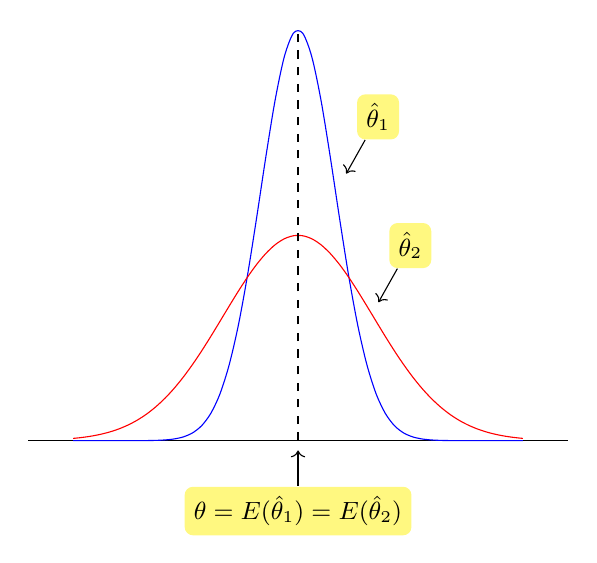
\begin{tikzpicture}[
every pin edge/.style={<-},
every pin/.style={fill=yellow!50,rectangle,rounded corners=3pt,font=\small}]
\begin{axis}[every axis plot post/.append style={
  mark=none,domain=-3:3,samples=50,smooth},
clip=false,
axis y line=none,
axis x line*=bottom,
ymin=0,
xtick=\empty,
]
\addplot {\gauss{0}{0.5}};
\addplot {\gauss{0}{1}};
\node[pin=70:{$\hat{\theta}_1$}] at (axis cs:0.57,0.5) {};
\node[pin=70:{$\hat{\theta}_2$}] at (axis cs:1,0.25) {};
\node[pin=270:{$\theta=E(\hat{\theta}_1)=E(\hat{\theta}_2)$}] at (axis cs:0,0) {};
\draw[dashed] (axis description cs:0.5,0) -- (axis description cs:0.5,0.92);
\end{axis}
\end{tikzpicture}
\end{center}

\noindent
If $T$ is a random variable with a pdf of the form \[ f_T(t) =  \begin{cases} 
      0 & \text{for } t < 0, \\
      \alpha e^{- \alpha t} & \text{for } t \geq 0.
      \end{cases} \] where $\alpha > 0$, then $T$ is an exponentially distributed random variable with parameter $\alpha$. $\prob{a \leq T \leq b} = \int_{a}^{b} \alpha e^{-\alpha t} dt = \big [ -e^{-\alpha t} \big ]_{a}^{b} = -e^{-a\alpha} - e^{-b \alpha }$.
      

\vspace{.3cm}
\noindent
If a random variable $X$ with pdf 

\begin{equation*}
f_X(x) = \frac{1}{\pi} \cdot \frac{1}{1 + (x-m)^2}
\end{equation*}

\noindent
where $x \in \R$, $m \in \R$ is Cauchy distributed with parameter $m$. The probability from $a$ to $b$ on a Cauchy distribution is found by $\int_{a}^{b} f_X(x) dx = \prob{a \leq X \leq b}$. 

\vspace{.3cm}
\noindent
Fix $a$ and $b$, $a < b$. Consider the experiment of choosing a number $X$ in the interval $(a, b)$. Then, $X$ has pdf \[ f_X(x) =  \begin{cases} 
      \frac{1}{b-a} & \text{for } a < x < b, \\
      0 & \text{for } x < a, x > b.
      \end{cases} \] X is \textbf{uniformly} distributed on $(a, b)$. Two properties shared by all pdfs $f(x)$ include 
    
\begin{enumerate}[label=(\roman*)]
\item $f(x) \geq 0$ for all $x$
\item $\int_{- \infty}^{\infty} f(x) dx = 1$.
\end{enumerate}

\noindent
When doing computations with normally distributed random variables, it helps to recall a result of Liouville's: For $a > 0$, 

\begin{equation*}
\int_{- \infty}^{\infty} e^{-ax^2} dx = \sqrt{\frac{\pi}{a}}.
\end{equation*}

\noindent
Clearly, for any $\mu \in \R$, 

\begin{equation*}
\int_{- \infty}^{\infty} e^{-a(x - \mu)^2} dx = \sqrt{\frac{\pi}{a}}.
\end{equation*}

\noindent
This is also valid for any $a \in \mathbb{C}$ for which Re$\{a\} < 0$. 

\nspace
\noindent
\textbf{Definition:} Random Variables$*$ $X$ and $Y$ are independent if $\prob{X \in A, Y \in B} = \prob{X \in A} \prob{Y \in B}$, for subset $A$ and $B$ of $\R$. $*$ We should say ``Jointly distributed random variables $X$ and $Y$.'' This means that $X$ and $Y$ are defined for the sample range and sample space. A family $\{ X_\lambda \}_{\lambda \in \Lambda}$ of (jointly distributed) random variables is independent if $\prob{X_{\lambda_1} \in A_1, X_{\lambda_2} \in A_2, \ldots, X_{\lambda_n} \in A_n }$ = $\prob{X_{\lambda_1} \in A_1} \cdot  \prob{X_{\lambda_2} \in A_2} \cdots \prob{X_{\lambda_n} \in A_n} $ for all finite subsets $\lambda_1, \lambda_2, \ldots, \lambda_n$ of $\Lambda$ and subsets $A_1, \ldots, A_n$ of $\R$.

\nspace
\noindent
Let $X$ be a random variable. The cumulative distribution function (cdf) of $X$ is $F_X(x) = \prob{X \leq x}$. Consider the Bernoulli variable $X$, where $X$ takes values $0$ and $1$, with $\prob{X = 0} = \prob{X = 1} = \frac{1}{2}$. 

%% TODO: add basic cdf function...

\noindent
This is the cdf of the discrete random variable $X$.

\begin{flushright}
\textbf{Date:} $10/12$
\end{flushright}

\noindent
For any random variable $X$, the cdf is $F_X (x) =  \prob{X \leq x}$. Suppose that $X$ is the Bernoulli variable assuming values $0$ and $1$, with probabilities $\alpha$ and $1-\alpha$.

\begin{equation*}
\prob{X = 0} = \alpha , \text{ } \prob{X = 1} = 1 - \alpha
\end{equation*}

\begin{tcolorbox}
\textbf{Example} Let $N$ be a Poisson-distributed random variable with parameter $\lambda > 0$. Then, $N$ assumes values in the range $\{ 0, 1, 2, \ldots \}$ with

\begin{equation*}
\prob{N = n} = \frac{\lambda^n}{n!} e^{- \lambda}.
\end{equation*}

%% TODO: Add a cdf graph of bernoulli variable x with \alpha and 1 - \alpha

\begin{center}
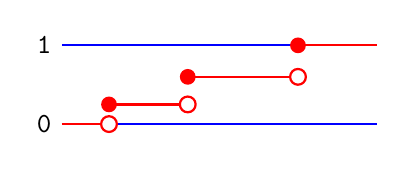
\begin{tikzpicture}[thick]
\draw[blue] (0,0) --  +(4,0) node[pos=0,left] {\tt\color{black} 1};
\draw[blue] (0,-1) -- +(4,0) node[pos=0,left] {\tt\color{black} 0};
\draw[red] (0,-1) -- (.6,-1) node[open] {};
\draw[red] (.6,-.75) node[closed] {} -- (1.6,-.75) node[open] {};
\draw[red] (1.6,-.4) node[closed] {} -- (3,-.4) node[open] {};
\draw[red] (3,0) node[closed] {} -- (4,0);
\end{tikzpicture}
\end{center}

\end{tcolorbox}

\noindent
Let $f$ be the continuous random variable $X$. Let $F(x) = \prob{X \leq x}$ be the cdf. For convenience, assume that $f(x)$ is continuous, except, possibly at finitely many points. Then, 

\begin{equation*}
F(x) = \prob{X \leq x} = \int_{- \infty}^{x} f(u) du.
\end{equation*}

\noindent
And by the Fundamental Theorem of Calculus, $F'(x) = f(x)$, where $f(x)$ is continuous. 

\begin{tcolorbox}
\textbf{Example} Let $T$ be exponentially distributed with parameter $\alpha > 0$. So, $T$ has pdf

\[ f(t) =  \begin{cases} 
      0 & \text{for } t < 0, \\
      \alpha e^{- \alpha t} & \text{for } t \geq 0.
      \end{cases} \]

% TODO: fix this image to match picture on phone
\begin{center}
\begin{tikzpicture}[
    declare function={gamma(\z)=
    (2.506628274631*sqrt(1/\z) + 0.20888568*(1/\z)^(1.5) + 0.00870357*(1/\z)^(2.5) - (174.2106599*(1/\z)^(3.5))/25920 - (715.6423511*(1/\z)^(4.5))/1244160)*exp((-ln(1/\z)-1)*\z);},
    declare function={gammapdf(\x,\k,\theta) = \x^(\k-1)*exp(-\x/\theta) / (\theta^\k*gamma(\k));}
]

\begin{axis}[
    axis lines=left,
    enlargelimits=upper,
    samples=50,
    legend entries={$k=1\quad \theta=2$,$k=2\quad \theta=2$, $k=9\quad \theta=0.5$}
]
\addplot [smooth, domain=0:20] {gammapdf(x,1,2)};
% \addplot [smooth, domain=0:20, red] {gammapdf(x,2,2)};
% \addplot [smooth, domain=0:20, blue] {gammapdf(x,9,0.5)};
\end{axis}
\end{tikzpicture}
\end{center}

% TODO: add a exponentially distributed pdf graph with y = f(t) [check pictures in phone]

What about the cdf?

\begin{equation*}
F(t) = \prob{T \leq t} = \int_{- \infty}^{t} f(s) ds.
\end{equation*}

Clearly, $F(t) = 0$ for $t < 0$. For $t \geq 0$, 

\begin{equation*}
F(t) = \int_{0}^{t} f(x) ds = 1 0 e^{- \alpha t}. 
\end{equation*}

% Add a graph of the cdf of exponentially distributed parameter [check phone for pictures]
\end{tcolorbox}

\begin{tcolorbox}
\textbf{Example} Let $X$ be a Cauchy-distributed with random variable with $m = 0$. Hence, $X$ has pdf

\begin{equation*}
f(x) = \frac{1}{\pi} + \frac{1}{1 + x^2}.
\end{equation*}

\noindent
The CDF is $F(x) = \int_{- \infty}^{\infty} f(u) du$, which is equal to 

\begin{align*}
& = \frac{1}{\pi} \int_{- \infty}^{x} \frac{1}{1+u^2} du \\
& = \frac{1}{\pi} \big [ \text{arctan}(x) - \text{arctan}(-\infty) \big ] \\
& = \frac{1}{\pi} \big [ \text{arctan}(x) \frac{\pi}{2} \big ].
\end{align*}

\noindent
$F(x)$, the CDF of the Cauchy variable $X$.

% Add a graph of the cdf of cauchy variable parameter [check phone for pictures]
\end{tcolorbox}

\noindent
\textbf{Properties of CDFs:} $F(x) = \prob{X \leq x}$

\begin{enumerate}
\item $\lim_{x \rightarrow - \infty} F(x) = 0$,
\item $\lim_{x \rightarrow \infty} F(x) = 1$,
\item $F(x)$ is non-decreasing,
\item $F(x)$ is right-continuous, i.e. $\lim_{h \rightarrow 0^{+}} F(x)$ at every $x$.
\end{enumerate}

\begin{tcolorbox}
\textbf{Example} Let $U$ be a uniformly distributed random variable on the interval $(a,b)$. So, $U$ has the pdf

\[ f(u) =  \begin{cases} 
      \frac{1}{b-a} & \text{for } a < u < b, \\
      0 & \text{for } u \leq a, \text{ } u \geq b.
      \end{cases} \]
 
\begin{center}
 \begin{tikzpicture}
\tkzInit[xmax=1,xstep=0.2,ymax=1,ystep=0.2]
\tkzDrawX[noticks,label={$x$}]
\tkzDrawY[noticks,label={$f_X(x)$}]
\tkzDefPoint(0.2,0.8){A}
\tkzDefPoint(0.8,0.8){B}
\tkzDefShiftPoint[A](-90:4){AB}
\tkzDefShiftPoint[B](-90:4){BB}
\tkzDefShiftPoint[AB](0:-0.6){ABL}
\tkzDefShiftPoint[BB](0:0.6){BBR}
\tkzPointShowCoord[xlabel=$a$,ylabel=$\frac{1}{b-a}$](A)
\tkzPointShowCoord[xlabel=$b$](B)
\tkzDrawSegments[color=cyan,thick](A,B AB,ABL BB,BBR)
\tkzDrawPoints[color=cyan,fill=cyan,size=6pt](A,B)
\tkzDrawPoints[color=cyan,fill=white,size=6pt](AB,BB)
\end{tikzpicture}
\end{center}

\noindent
The CDF is then 

\[ F(u) = \prob{U \leq u} = \int_{- \infty}^{u} f(v) dv =  \begin{cases} 
	  0 & \text{for } u \leq a, \\
      \frac{u-a}{u-b} & \text{for } a < u < b, \\
      1 & \text{for } u \geq b.
      \end{cases} \]
      
% TODO: Add a cdf graph for uniform distribution here
\end{tcolorbox}

\noindent
$\prob{X \leq x}$. We assign a probability to the event $(X \leq x)$. Think of $X$ as a function on a sample space $\Omega$,

\begin{equation*}
X : \Omega \rightarrow \R.
\end{equation*}

% TODO: add picture here from phone on x = X(\omega)

\noindent
For any $x$, we'll write $(X \leq x)$ for the set $\big \{ \omega \in \Omega \lvert X(\omega) \leq x \big \}$. \textbf{Question:} For a CAPs $\faps$, is the subset $(X \leq x)$ an event, i.e. is $(X \leq x \in \field$? $($Here $\field$ is the $\sigma$-field of events.$)$ 

\noindent
\textbf{Example:} Consider the sample space $\Omega = \{ 1,2,3,4,5 \}$. Let $A=\{ 1,2 \}$, $B =\{ 3,4 \}$, and $C =\{ 5 \}$. Let $\field$ be the field (actually a $\sigma$-field) of events,

\begin{equation*}
\big \{ \emptyset, A, B, C, A+B, B+C, A+C, \Omega \big \}.
\end{equation*}

\noindent
Let $X : \Omega \rightarrow \R$ by $X(\omega) = \omega$. The subset $(X \leq 3)$ is $\{ 1,2,3 \} \not \in \field$. Hence, $\prob{X \leq 3}$ is undefined for the CAPS $\faps$.

\nspace
\noindent
\textbf{Definition:} Let $\faps$ be a CAPs. So, $\field$ is a $\sigma$-field of subsets of $\Omega$. A random variable is a function $X : \Omega \rightarrow \R$ such that for every $x \in \R$, $(X \leq x) \in \field$. So, $X$ is an $\field$-measurable function. 

\noindent
Let $X$ be a random variable. So, for every $x$, $(X \leq x) \in \field$. Observe that $(x < X) = (X \leq x)$. So, because $\field$ is closed under complementation, $(x < X)$ is an event. What about $(X < x)$? Well,

\begin{equation*}
(X < x) = \bigcup_{n=1}^{\infty} (X \leq x - \frac{1}{n}) \in \field
\end{equation*}

\noindent
because $\field$ is closed under countable union. By another complementation argument,  

\begin{equation}
(x \leq X) \in \field.
\end{equation}
% <--\in \field for ever n

\noindent
By similar arguments, $(a < X \leq b)$, $(a < X \leq b)$, and $(a < X \leq b)$ lie in $\field$ also. So, for any interval $I$, $(X \in I) \in \field$. For $(a < X \leq b)$,
$(a < X \leq b) = \big ( (X \leq b) \in \field \cap (X > a) \in \field \big ) \in \field$ also.

\begin{flushright}
\textbf{Date:} $10/19$
\end{flushright}

\nspace
\noindent
We have a CAPs $\faps$. A random variable $X$ is a function, 

\begin{equation*}
X: \Omega \rightarrow \R
\end{equation*}

\noindent
satisfying the condition $\{ \omega \in \Omega \text{ } \lvert \text{ } X(\omega) \leq x \}$ for ever $x \in \R$ Because $(X \leq x) \in \field$ for every $x \in \R$, $X$ is called $\field$-measurable. So, a random variable is an $\field$-measurable function on $\Omega$. Let $X$ be a random variable. We showed that for every interval $I$, $\{ \omega \in \Omega \text{ } \lvert \text{ } X(\omega) \in I \} = (X \in I) \in \field$. Let $A \subset \R$ be a set that could be ``manufactured'' by countably many union, intersection, and complementation operations, starting with intervals. Then, by the countable additivity of $P$, the face that $\field$ is a $\sigma$-field, and the $\field$-measurability of $X$, $(X \in A) \in \field$.

\nspace
\noindent
The set of all subsets $A$ of $\R$ that can be constructed in this manner is itself a $\sigma$-field. It is called the Borel $\sigma$-field. So, for every $A \in \mathcal{B}$, the Borel $\sigma$-field, $(X \in A) \in \field$. Alternative \textbf{definition}: $X: \Omega \rightarrow \R$ is $\field$-measurable if $(X \in A) \in \field$ for every Borel subset $A$ of $\R$. A rigorous definition of the Borel $\sigma$-field,

\begin{enumerate}[label=(\roman*)]
\item Let $\big \{ \field_{\lambda} \big \}_{\lambda \in \Lambda}$ be a family of $\sigma$-fields. Then, $\bigcap_{\lambda \in \Lambda} \field_{\lambda}$ is itself a $\sigma$-field.
\item Let $\big \{ \mathcal{B}_{\lambda} \big \}_{\lambda \in \Lambda}$ be the class of all $\sigma$-fields of subsets of $\R$ that include all intervals of the form $(- \infty, x ]$.
\item Thus, $\bigcap_{\lambda \in \Lambda} \mathcal{B}_{\lambda}$ is itself a $\sigma$-field that contains all subsets of $\R$ of the form $(- \infty, x ]$. In fact, $\bigcap_{\lambda \in \Lambda} \mathcal{B}_{\lambda}$ is the smallest $\sigma$-field that contains these intervals. We define $\mathcal{B} = \bigcap_{\lambda \in \Lambda} \mathcal{B}_{\lambda}$. Thus, the Borel $\sigma$-field is the smallest $\sigma$-field that contains all sets of the form $( - \infty, x] \subset \R$.
\end{enumerate}

\nline
Grinstead and Snell $4.1$: Consider a discrete sample space $\Omega$. Recall that a distribution function (df) $m$ on $\Omega$ is a function

\begin{equation*}
m : \Omega \rightarrow [0,1]
\end{equation*}

\noindent
such that $\sum_{\omega \in \Omega} m(\omega) = 1$. Let $X$ be a random variable on $\Omega$ (so, $X$ is discrete) with range $\{ x_i \}_{i \in I}$ where $I$ is a countable index set. The probability mass function (pmf) $p: \{ x_i \}_{i \in I} \rightarrow [0,1]$ by $p(x_i) = \prob{X = x_i}$. Hence, 

\begin{equation*}
p(x_i) = \prob{X = x_i} = \sum_{\omega \in (X = x_i)} m(\omega).
\end{equation*}

\noindent
Throw a fair die twice. Thus, $\Omega = \Big \{ (1,1), (1,2), \ldots, (6,6), \Big \}$. So, $\lvert \Omega \rvert = 36$, and we use the distribution function $m : \Omega \rightarrow [0,1]$ by $m(\omega) = \frac{1}{36}$. Define $X$ to be the sum of the two throws. Thus, for $\omega = (\omega_1, \omega_2)$, $X(\omega) = \omega_1 + \omega_2$. The pmf of $X$ is 

\begin{align*}
p(2) & = \prob{X = 2} = \frac{1}{36} \\
p(3) & = \prob{X = 3} = m(1,2) + m(2,1) = \frac{1}{18} \\
p(4) & = \prob{X = 4} = m(1,3) + m(2,2) + m(3,1) = \frac{1}{12} \\
& \hspace*{3cm} \vdots \\
p(12) & = \prob{X = 12} = m(6,6) = \frac{1}{36} \\
\end{align*}

\noindent
For discrete sample spaces and random variables, we have distribution functions an probability mass functions. For continuous random variables, we have probability distribution functions. For all random variables, we have cumulative distribution functions. 

\nline
Let $X$ and $Y$ be jointly distributed random variables, i.e. random variables on the same CAPs $\faps$. Suppose that $X$ and $y$ are discrete, with ranges $\{ x_i \}$ and $\{ y_j \}$ respectively. The joint pmf of $X$ and $Y$ is $p(x_i, y_j) = \prob{ X = x_i, Y = y_j} = \sum_{\omega \in (X = x_i, Y = y_j)} m(\omega)$. The conditional probability that $X = x_i$, given $Y=y_j$ is

\begin{equation*}
\frac{\prob{X = x_i, Y = y_j}}{\prob{Y = y_j}}.
\end{equation*} 

\noindent
The joint probability mass function of $X$ and $Y$ is $p(x_i, y_j) = \prob{X = x_i, Y = y_j}$. Let $p_X$ and $p_Y$ be the probability mass functions of $X$ and $Y$ respectively. Then, 

\begin{align*}
p_X = \prob{X = x_i} & = \sum_{j} \prob{X = x_i, Y = y_j} \\
& = \sum_{j} p(x_i, y_j) \\
\end{align*}

\noindent
and, 

\begin{align*}
p_Y = \prob{Y = y_j} & = \sum_{i} \prob{X = x_i, Y = y_j} \\
& = \sum_{j} p(x_i, y_j) \\
\end{align*}

\noindent
In this context, $p$ is the joint probability mass function and $p_X$ and $p_Y$ are the marginal probability mass functions. Let $p_{X \lvert Y} (x_i \lvert y_j) = \prob{X = x_i \lvert Y = y_j}$. Then, $p_{X \lvert Y} (x_i \lvert y_j) = \frac{p(x_i, y_j)}{p_Y (y_j)}$. $p_{X \lvert Y}$ is the conditional probability mass function of $X$ given $Y$.

\nline
If $X$ and $Y$ are independent, then $p(x_i, y_j) = p_X(x_i) p_Y(y_j)$. Why? Well, 

\begin{align*}
p(x_i, y_j) & = \prob{X = x_i, Y = y_j } \\
& = \prob{X = x_i} \prob{Y = y_j} \\
& = p_X(x_i) p_Y(y_j). 
\end{align*}

\nline
Let $X$ and $Y$ be jointly distributed, continuous random variables. The joint probability density function of $X$ and $Y$ is the function $f : \R^2 \rightarrow \R$ defined by

\begin{equation*}
\prob{X \leq a, Y \leq b} = \int_{- \infty}^{b} \int_{- \infty}^{a} f(x, y) dx \text{ } dy.
\end{equation*}

\noindent
More generally, 

\begin{equation*}
\prob{X \in A, Y \in B} = \int_{B} \int_{A} f(x, y) dx \text{ } dy. 
\end{equation*}

\noindent
Let $a$ and $a$ be the probability dis

% ================================================================================================================================
% ================================================================================================================================

\begin{flushright}
\textbf{Date:} $10/24$
\end{flushright}

% Grinstead and Snell section 4.2, 4.3

Let $X$ be a discrete random variable with range $\{ x_i \}$. The pmf of $X$ is 

\begin{equation}
\mathbb{P}_X(x) = \begin{cases} 
	  \prob{X = x} & \text{for $x$ in the range of } X, \\
      0 & \text{if } a = 0 \text{for $x$ not in the range of } X. \\
      \end{cases}
\end{equation}

\noindent
Thus, $p_X(x_i) = \prob{X = x_i}$. If $X$ and $Y$ are discrete (jointly distributed) random variables, then their joint probability mass function is $\prob{x_i, y_j} = \prob{X = x_i, Y=y_j}$. The marginal probability mass functions are then $\mathbb{P}_X{x_i} = \sum_{j} \prob{x_i, y_j}$ and $\mathbb{P}_Y(y_j) = \sum_{i} \prob{x_i, y_j}$. The conditional probability mass function of $X$ given $Y=y_j$ is 

\begin{equation*}
p_{X \lvert Y} (x_i \lvert y_j) = \frac{p(x_i, y_j}{p_Y(y_j)}.
\end{equation*}

% todo: insert table from pictures

\noindent
Thus $p(1,4) = \prob{X = 1, Y = 4} = .1$. The marginal probability mass function of $Y$ is 

\begin{align*}
\mathbb{P}_Y = \prob{Y = 2} & = \prob{X=0, Y=2} + \prob{X=1, Y=2} + \prob{X=2, Y=2} \\
& = \prob{X=0, Y=2} + \prob{X=1, Y=2} + \prob{X=2, Y=2} \\ 
& = .35
\end{align*}

\noindent
Similarly, $P\mathbb{P}_Y (3) = .35$ and  $P\mathbb{P}_Y (4) = .4$. Now, what is $p_{X \lvert Y} (x \lvert 2)$?

\begin{align*}
p_{X \lvert Y} (0 \lvert 2) = \frac{.15}{.35} = \frac{3}{7} && p_{X \lvert Y} (1 \lvert 2)  = \frac{.1}{.35} = \frac{2}{7} && p_{X \lvert Y} (2 \lvert 2) = \frac{.1}{.35} = \frac{2}{7}
\end{align*}

% Get notes from random erase form cooper....

\noindent
Let $\{ X_\lambda \}_{\lambda \in \Lambda}$ be a set of jointly distributed random variables. The $X_\lambda$ are independent if for every finite subset $\lambda_1, \ldots, \lambda_n$ of $\Lambda$, $\prob{X_{\lambda_1} \in B_1, \ldots, X_{\lambda_n} \in B_n} = \prob{X_{\lambda_1} \in B_1} \cdots \prob{X_{\lambda_n} \in B_n}$. Back to the case of discrete, independent random variables $X$ and $Y$, with ranges $\{ x_i \}$ and $\{ y_j \}$ (subsets with $1$ point each). Then,

\begin{align*}
p(x_i, y_j) = \prob{X = x_i, Y=y_j} & = \prob{X \in \{ x_i \} , Y \in \{ y_j \}} \\
&= \prob{X = x_i} \cdot \prob{ Y=y_j} \\
&= \mathbb{P}_X(x_i) \cdot  \mathbb{P}_Y(y_j).
\end{align*}

\begin{center}
\textbf{Continuous Conditional Probability}
\end{center}

\noindent
Let $X$ and $Y$ be continuous random variables with joint probability distribution function $f(x,y)$. So,

\begin{equation*}
\prob{a < X \leq b, c < Y \leq d} = \int_{c}^{d} \int_{a}^{b} f(x,y) dx \text{ } dy
\end{equation*}

\noindent
More generally, let $B \subset \R^2$. Then,

\begin{equation*}
\prob{(X, Y) \in B} = \iint_B f(x,y) dA.
\end{equation*}

\noindent
Clearly, $\iint_{\R^2} f(x,y) dA = 1$.

% insert graph from phone with blob B and shaded in

\noindent
Conditional probability distribution functions: We'd like t define $f_{X \lvert Y}(x \lvert y)$, the conditional probability distribution function of $X$ given $Y=y$. How do we do this, given $\prob{Y = y} = 0$ for a continuous variable $Y$? Start with $\prob{a < X \leq b \lvert Y = y }$. Assume that this expression is well-defined in some sense. Then, it should be that

\begin{align*}
\prob{a < X \leq b \lvert Y = y} &= \lim_{h \rightarrow 0^{+}} \prob{a < X \leq b \lvert y \leq Y \leq y+h} \\
&= \lim_{h \rightarrow 0^{+}} \frac{ \prob{a < X \leq b, y \leq Y \leq y+h}}{\prob{y \leq Y \leq y+h}} \\
&= \lim_{h \rightarrow 0^{+}} \frac{ \frac{1}{h} \int_{a}^{b} \int_{y}^{y+h} f(x, \eta) d \eta \text{ } dx}{ \frac{1}{h} \int_{y}^{y+h} f_Y(\eta) d \eta } \\
&= \frac{\int_{a}^{b} f(x, y) dx }{f_Y(y)}\\
&= \int_{a}^{b} \frac{ f(x, y)}{f_Y(y)} dx. \\
\end{align*}

\noindent
Thus, $\frac{ f(x, y)}{f_Y(y)} = f_{X \lvert Y} (x \lvert y)$ is the conditional probability distribution function of $X$ given $Y=y$. Clearly, $f_{X \lvert Y} (x \lvert y)$, (as a function of $x$) is non-negative, and 

\begin{align*}
\int_{- \infty}^{\infty} f_{X \lvert Y} (x \lvert y) dx & = \int_{- \infty}^{\infty} \frac{f(x,y)}{f_Y(y)} dx \\
&= \frac{1}{f_Y(y)} \int_{- \infty}^{\infty} f(x,y) dx \\
&= \frac{f_Y(y)}{f_Y(y)} = 1 
\end{align*}

\noindent
Thus, $f_{X \lvert Y} (x \lvert y)$ at fixed $y$, is a pdf, as a function of $x$. We have the law of total probability in the continuous case

\begin{align*}
\prob{a < X \leq b } = \prob{a < X \leq b, - \infty < Y < \infty} &= \int_{a}^{b} \int_{- \infty}^{\infty} f(x,y) dy \text{ } dx \\
&= \int_{a}^{b} \int_{- \infty}^{\infty} \frac{f(x,y)}{f_Y(y)} f_Y(y) dy \text{ } dx \\
&= \int_{a}^{b} \int_{- \infty}^{\infty} f_{X \lvert Y} (x \lvert y) \cdot f_Y(y) dy \text{ } dx \\
&= \int_{- \infty}^{\infty} \int_{a}^{b} f_{X \lvert Y} (x \lvert y) dx \cdot f_Y(y) dy \\
&= \int_{- \infty}^{\infty} \prob{a < X \leq b \lvert Y = y} \cdot f_Y(y) dy
\end{align*}

\noindent
Suppose now that $X$ and $Y$ are independent random variables. Then, $\prob{a < X \leq b, c < Y \leq d} = \prob{a < X \leq b} \cdot \prob{c < Y \leq d}$. Thus,

\begin{align*}
\int_{a}^{b} \int_{c}^{d} f(x,y) dy \text{ } dx = \int_{a}^{b} f_X(x) dx \int_{c}^{d} f_Y(y) dy = \int_{a}^{b} \int_{c}^{d} f_X(x) \cdot f_Y(y) dy \text{ } dx.
\end{align*}

\noindent
Thus, $f(x,y) = f_X(x) \cdot f_Y(y)$. This extends in the obvious way to independent, continuous random variables $X_1, \ldots, X_n$. For any jointly distributed random variables $X_1, \ldots, X_n$, the joint cumulative distribution function is $F(x_1, \ldots, x_n) = \prob{X_1 \leq x_1, \ldots, X_n \leq x_n}$. Suppose that the $x_j$ are continuous, with joint probability distribution function $f(x_1, \ldots, x_n)$. Then, 

\begin{align*}
F(x_1, \ldots, x_n) &= \prob{X_1 \leq x_1, \ldots, X_n \leq x_n} \\
&= \int_{- \infty}^{x_n} \int_{- \infty}^{x_{n-1}} \cdots \int_{- \infty}^{x_{1}} f(u_1, \ldots, u_n) du_1 \ldots du_n
\end{align*}

\noindent
Thus, $f(x_1, \ldots, x_n) = \frac{\partial^n}{\partial x_1 \partial x_2 \cdots \partial x_n} F(x_1, \ldots, x_n)$.

\nline
Let $X_1, \ldots, X_n$ be random variables with cumulative distribution function $F(x_1, \ldots, x_n)$ and marginal cumulative distribution functions $f_{X_i} (x_i)$. If $f(x_1, \ldots, x_n)$ is the joint probability distribution function, then $\frac{\partial^n}{\partial x_1 \partial x_2 \cdots \partial x_n} F(x_1, \ldots, x_n) = f(x_1, \ldots, x_n)$. Finally, if $X_1, \ldots, X_n$ are independent, then 

\begin{equation*}
F(x_1, \ldots, x_n) = \prob{X_1 \leq x_1, \ldots, X_n \leq x_n} = \prob{X_1 \leq x_1} \cdots \prob{X_n \leq x_n} = F_{X_1} (x_1) \cdots F_{X_n} (x_n).
\end{equation*}

\begin{tcolorbox}
\noindent
\textbf{Example:} Let $X$ and $Y$ be continuous random variables with joint probability density function

\[ f(x,y) = \begin{cases} 
	  x^2 + xy + \frac{5}{4} y^2 & \text{ } 0 < x < 1 \text{ and } 0 < y < 1, \\
      0 & \text{ otherwise}. \\
      \end{cases} \]
 
\noindent
Say we want to find $\prob{X < Y}$. Then, $\prob{X < Y} = \mathbb{P} \Big ( (X, Y) \in T \Big )$. Formally, we know that this is equivalent to

\begin{align*}
\mathbb{P} \Big ( (X, Y) \in T \Big ) &= \int_{0}^{1} \int_{x=0}^{x=y} (x^2 + xy + \frac{5}{4} y^2) dx \text{ } dy \\
& = \int_{0}^{1} (\frac{1}{3} y^3 + \frac{1}{2} y^3 + \frac{5}{4} y^3) dy \\
&= \frac{25}{12} \int_{0}^{1} y^3 dy \\
&= \frac{25}{48}.
\end{align*}

\noindent
Find the marginal probability distribution function $f_Y$ of $Y$. We see that 

\begin{align*}
f_Y (y) &= \int_{- \infty}^{\infty} f(x,y) dx \\
&= \int_{- \infty}^{\infty} (x^2 + xy + \frac{5}{4} y^2) dx \\ 
&= \frac{1}{3} + \frac{1}{2} y + \frac{5}{4} y^2 \text{, for } 0 < y < 1.
\end{align*}

\noindent
Hence, at fixed $y \in (0,1)$, the conditional probability distribution function of $X$, given $Y=y$ is. 

\[ f_{X \lvert Y} (x \lvert y) = \frac{f(x,y)}{f_Y(y)} = \begin{cases} 
	  0 & \text{ for } x \leq 0, \text{ } x \geq 1, \\
      \frac{x^2 + xy + \frac{5}{4} y^2}{\frac{1}{3} + \frac{1}{2} y + \frac{5}{4} y^2} & \text{ for } 0 < x < 1. \\
      \end{cases} \]
\end{tcolorbox}

\subsection*{Expected Value}
Let $X$ be a discrete random variable on a discrete sample space $\Omega$. The expected value or expectation of $X$ (or the mean of $X$) is the average value of $X$, taken over $\Omega$. The E$(X) = \sum_{\omega \in \Omega} X(\omega) m(\omega)$, where $m$ is the distribution function on $\Omega$. \textbf{Note:} $m$ is valid as a distribution function here because the sample space is discrete. A \textbf{more useful} expression is based on the probability mass function $p_X(x_i)$. Let $\{ x_i \}$ be the range of $X$. Then, the expected value of $X$ is E$(X) = \sum_{\omega \in \Omega} X(\omega) m(\omega) = \sum_{i} \sum_{X = x_i} X(\omega) m(\omega) = \sum_{i} \sum_{X = x_i} m(\omega) = \sum_{i} \prob{X = x_i} = \sum_{i} x_i p_X (x_i)$. Here, the constraint on the second summation is really `` for every $i$, $X = x_i$'', which is equivalent to $\{ \omega \in \Omega \lvert X(\omega) = x_i \}$. 

\nline
Suppose now that $X$ is a continuous random variable with probability distribution function $f_X (x)$. In this case, a simple limiting argument yields the formula E$(X) = \int_{- \infty}^{\infty} x f_x (x) dx$. Should the sum or integral diverge, the random variable $X$ is said to have no expected value.

\nline
\textbf{Example}: Let $X$ be a Bernoulli variable with range $\{ x_1, x_2 \}$ and probability mass function $p_X (x_1) = \alpha_1$, $p_X (x_2) = \alpha_2$, $\alpha_1 + \alpha_2 = 1$. Then, $X$ has mean E$(X) = \alpha_1 x_1 + \alpha_2 x_2$.

\nline
\textbf{Example}: We are flipping a coin until a tail occurs. Let $P(H)=p$, $P(T)=1-p$, $0 < p < 1$. Let $N$ be the number of the trial in which the $T$ occurs. Then, $N$ is geometrically distributed:

\begin{align*}
p_N(n) = P(N=n) = p^{n-1} (1-p), \textbf{ } n=1,2,3, \ldots
\end{align*}

\noindent
Then, E$(N) = \sum_{n=1}^{\infty} n p_N(n) = \sum_{n=1}^{\infty} n p^{n-1} (1-p) = (1-p) \frac{d}{dp} \sum_{n=0}^{\infty} p^n = (1-p) \frac{d}{dp} \frac{1}{1-p} = \frac{1}{1-p}$.

\noindent
\textbf{Example}: Let $X$ be Poisson-distributed with parameter $\lambda > 0$. So, $X$ has range $\{ 0, 1, 2, 3, \ldots \}$ and probability mass function $f_X(k) = \frac{\lambda^k}{k!	} e^{- \lambda}$. Then, E$(X) = \sum_{k=0}^{\infty} k p_X(k) = \sum_{k=1}^{\infty} k \cdot \frac{\lambda^k}{k!	} e^{- \lambda} = \lambda e^{- \lambda} \cdot e^{- \lambda} = \lambda$. So, E$(X) = \lambda$ is the mean occurrence rate.

\nline
Let $Y$ be Cauchy-distributed with parameters $m=0$. $Y$ has probability distribution function $f_Y (y) = \frac{1}{\pi} \cdot \frac{1}{1+(y-m)^2} = \frac{1}{1+y^2} \cdot \frac{1}{\pi}$, when $m=0$. Hence 

\begin{align*}
\text{E}(Y) = \int_{- \infty}^{\infty} y f_Y(y) dy &= \frac{1}{\pi} \int_{- \infty}^{\infty} \frac{y}{1+y^2} dy \\
&= \lim_{a \rightarrow \infty, \text{ } b \rightarrow \infty} \frac{1}{\pi} \int_{0}^{a} \frac{y}{1+y^2} dy + \frac{1}{\pi} \int_{-b}^{\infty} \frac{y}{1+y^2} dy \\
&= lim_{a \rightarrow \infty} \frac{1}{\pi} \int_{0}^{\infty} \frac{y}{1+y^2} dy \\
&= lim_{a \rightarrow \infty} \frac{1}{2 \pi} \text{ln}(1+a^2) = \infty.
\end{align*}

\noindent
So, the integral diverges, and we conclude that E$(X)$ does not exist for the Cauchy distribution. 

\nline
Let $X$ be normaly distributed with parameters $\mu$, $\sigma$. So, $X$ has the probability distribution function $f_X(x) = \frac{1}{\sqrt{2 \pi \sigma^2} e^{-\frac{(x-\mu)^2}{2 \sigma^2}}}$, $\mu \in \R$, $\sigma > 0$. E$(X) = \frac{1}{\sqrt{2 \pi \sigma^2}} \int_{- \infty}^{\infty} x e^{-\frac{(x-\mu)^2}{2 \sigma^2}} dx$. Set $z = \frac{x-\mu}{\sigma}$. So, $dx = \sigma dz$, and the integral becomes:

\begin{align*}
\frac{1}{\sqrt{2 \pi \sigma^2}} \Big [ \int_{- \infty}^{\infty} \sigma z e^{- \frac{z^2}{2} \cdot \sigma dz}+ \mu \int_{- \infty}^{\infty} \sigma z e^{- \frac{z^2}{2}} \cdot \sigma dz \Big ]
\end{align*}

\noindent
The first term is equal to $0$, and the second term is equal to $\sigma \mu \sqrt{2 \pi}$ from Liouville's formula. 

\begin{flushright}
\textbf{Date}: $10/31$
\end{flushright}

\nline
For $X$ discrete with range $\{ x_i \}$, E$[X] = \sum_{\Omega} = X( \omega )m( \omega ) = \sum_{i} x_i p_x (x_i)$, where $m$ is the $df$ on $\Omega$ and $p_x$ the probability mass function of $x$. For a continuous $x$, E$[X]= \int_{- \infty}^{\infty} x f_X(x) \text{ } dx$ where $f_X$ is the probability distribution function of $X$. 

\nline
\textit{Properties of expectations}: Let $X$ be a random variable and $g : \R \rightarrow \R$ be continuous. Then, $Y = g(X)$ is also a random variable. What is E$[X] =$ E$[g(X)]$? Suppose that $X$ is discrete with probability mass function $p_X$. Let $m$ be a $df$ on $\Omega$. Then, by definition, E$[Y] = \sum_{\Omega} g(X(\omega)) m(\omega) = \sum_{i} \sum_{x = x_i} g(X(\omega)) m(\omega) = \sum_{i} \sum_{x = x_i} g(x_i) m(\omega) = \sum_{i} g(x_i) \sum_{x = x_i} m(\omega) = \sum_{i} g(x_i) \mathbb{P}(X = x_i) = \sum_{i} g(x_i) p_X(x_i)$.

\nline
For a continuous random variable $X$, with probability distribution function $f_X$, E$[g(X)] = \int_{- \infty}^{\infty} g(x) f_X (x) \text{ } dx$. 

\begin{tcolorbox}
Let $T$ be exponentially distributed with probability distribution function 

\[ f_T(t) = \frac{f(x,y)}{f_Y(y)} = \begin{cases} 
	  0 & \text{ for } t < 0, \text{ wher } \alpha > 0. \\
      \alpha e^{- \alpha t} & \text{ for } t \geq 0. \\
      \end{cases} \]
      
\nline
Then, we see that

\begin{align*}
\text{E}[T] = \int_{- \infty}^{\infty} t f_T (t) \text{ } dt &= \int_{0}^{\infty} \alpha t e^{- \alpha t} \text{ } dt \\
&= \int_{0}^{\infty} t d \big ( e^{- \alpha t} \big ) = \Bigg [ -t e^{- \alpha t} \Bigg ]_{0}^{\infty} + \int_{0}^{\infty} e^{- \alpha t} \text{ } dt \\
&= \Bigg [ \frac{e^{- \alpha t}}{- \alpha} \Bigg ]_{0}^{\infty} = \frac{1}{\alpha}.
\end{align*}

Let $g(u) = e^{- u}$. The expected value of the random variable $Y = g(T) = e^{-T}$ is E$[Y]=$E$[g(T)] = \int_{- \infty}^{\infty} g(t) f_T (t) \text{ } dt = \int_{0}^{\infty}e^{-t} e^{- \alpha t} \text{ }  dt \cdot \alpha = \alpha \int_{0}^{\infty} e^{-(1 + \alpha) t} dt = \frac{\alpha}{1 + \alpha}$.

\nline
Next, let $c$ be any constant and $g : \R \rightarrow \R$ by $g(u) = cu$. Then (for $X$ discrete), E$[cX] = $E$[g(X)] = \sum_{i} g(x_i) f_X(x_i) = \sum_{i} c x_i f_X (x_i) = c \sum_{i} x_i f_X(x_i) = c \text{E}[X]$. The same result is valid for the continuous case: E$[cX]=c$E$[X]$.
\end{tcolorbox}

\nline
Let $g : \R^2 \rightarrow \R$ be continuous. Let $X$ and $Y$ be jointly distributed random variables. What is E$\big [ g(X,Y) \big ]$? Let $Z = g(X,Y)$. Assume that $X$ and $Y$ are discrete with ranges $\{ x_i \}$ and $\{ y_i \}$ respectively and joint probability mass function $f$. Then, E$[Z] = \text{E}[g(X,Y)] = \sum_{\Omega} g(X(\omega), Y(\omega)) m(\omega)$. Let $A_{ij}$ be the event $(X = x_i, Y = y_j)$. [\textbf{Note}: $A_{ij}$ is just the intersection of the events $X=x_i$ and $Y=y_j$ because both are Borel subsets the real number line, and thus subsets of $\Omega$]. Then, by E$[Z] = \text{E}[g(X,Y)]$, $\text{E}[g(X,Y)] = \sum_{i} \sum_{j} \sum_{A_{ij}} g(X(\omega), Y(\omega)) m(\omega) = \sum_{i} \sum_{j} g(x_i, y_j) \sum_{A_{ij}} m(\omega) = \sum_{i} \sum_{j} g(x_i, y_j) \prob{m(\omega} = \sum_{i} \sum_{j} g(x_i, y_j) p(x_i, y_j)$.

%% TODO: double check statement about borel subsets above


In the continuous case, E$\int_{- \infty}^{\infty} \int_{- \infty}^{\infty} g(x,y) f(x,y) \text{ } dxdy$, where $f$ is the joint probability distribution function. Special case: $g(u,v) = u+v$. Then, E$\Big [ g(X,Y) \Big ] = \text{E}\Big [ X + Y \Big ] = \sum_{\Omega} \Big [ X(\omega) + Y(\omega) \Big ] m(\omega) = \sum_{\Omega}  X(\omega) m(\omega) + \sum_{\Omega} Y(\omega) m(\omega) = \text{E}\Big [ X \Big ] + \text{E}\Big [ Y \Big ] = \sum_{i} x_i p_X (x_i) + \sum_{j} y_j p_Y (y_j)$. The same holds in the case of continuous variables. Combine two results: Let $X$ and $Y$ be jointly distributed random variables, and $a$ and $b$ constants. Then, $\text{E} \Big [ aX + bY \Big] = a \text{E} [ X \Big] + b \text{E}[ Y \Big]$.

\nline
Let $X$ and $Y$ be independent, jointly distributed random variables. Then, $\text{E} \Big [ XY \Big] = \text{E} \Big [ X \Big] \cdot \text{E} \Big [ Y \Big] $. Suppose that $X$ and $Y$ are continuous, with joint probability distribution function $f$. Let $g : \R^2 \rightarrow \R$ by $g(u,v) = uv$. Then, $\text{E} \Big [ XY \Big] = \text{E} \Big [ g(X,Y) \Big] = \int_{- \infty}^{\infty} \int_{- \infty}^{\infty} g(x,y) f(x,y) \text{ } dx \text{ } dy$.

%%% TODO: insert material from thursday november, 2nd

\begin{flushright}
\textbf{Date:} $11/7$
\end{flushright}

\nline
Let $X$ be binomially distributed with parameters $n,p$: $P(X = k) = p_X(k) = {n \choose k} p^k (1-p)^{n-k}$, $k=0,1,2, \ldots, n$. We already know that $\expected{X} = np$. Then, 

\begin{align*}
\expected{X^2} &= \sum_{k = 0}^{n} k^2 {n \choose k} p^k (1-p)^{n-k} \\
&= \sum_{k = 1}^{n} (k^2-k+k) {n \choose k} p^k (1-p)^{n-k} \\
&= \sum_{k = 2}^{n} (k^2-k) {n \choose k} p^k (1-p)^{n-k} + \sum_{k = 0}^{n} k {n \choose k} p^k (1-p)^{n-k} \\
&= \Bigg [ \sum_{k = 2}^{n} k(k-1) \frac{n!}{(n-k)!k!} p^k (1-p)^{n-k} \Bigg ] + np \\
&= \Bigg [  n(n-1)p^2 \sum_{k = 2}^{n} k(k-1)p^{k-2} \frac{(n-2)!}{(n-k)!k!} (1-p)^{n-k} \Bigg ] + np \\
&= \Bigg [  n(n-1)p^2 \sum_{k = 2}^{n} k(k-1)p^{2} \frac{(n-2)!}{(k-2)! \big [ (n-2)-(k-2) \big ]!} p^{k-2} (1-p)^{(n-2)-(k-2)} \Bigg ] + np, n-2=m, k-2=l \\
&= \Bigg [ n(n-1)p^2 \sum_{l = 0}^{m} {m \choose l} p^l (1-p)^{m-l} \Bigg ] + np \\
&= n(n-1)p^2 + np \\
\end{align*}

\nline
So, $\variance{X} = \expected{X^2} - \expected{X}^2 = n(n-1)p^2 + np - n^2p^2 = np-np^2 = np(1-p)$. Another method to approach this is to define the indicator, or ``counter'' variables $X_1, \ldots, X_n$ by 

\[ X_j =  \begin{cases} 
      1& \text{if ``H'' on flip } j, \\
      0 & \text{if ``T'' on flip } j.
      \end{cases} \]

\nline
The $X_j$ above are $iid$ (independent, identically distributed) random variables. 

\nline
\textbf{Chebyshev's Inequality}: Let $X$ be a random variable with $\expected{X} = \mu$ and $\variance{X} = \sigma^2$. For $\epsilon > 0$, what is $\prob{\lvert x - \mu \rvert \geq \epsilon}$? Clearly this depends on $X$. Chebyshev's inequality is an estimate of this probability: $\prob{\lvert x - \mu \rvert \geq \epsilon} \leq \frac{\sigma^2}{\epsilon^2}$.

\begin{tcolorbox}
\textbf{Proof} Let's take (WLOG) $X$ to be continuous with pdf $f_X$. Then, 

\begin{align*}
\sigma^2 = \variance{X} &= \expected{\big [ (X - \mu)^2 \big ]} \\
&= \int_{- \infty}^{\infty} (x- \mu)^2 f_X(x) dx \\
& \geq \int_{\lvert x - \mu \rvert \geq \epsilon} (x- \mu)^2 f_x(x) dx \\
& \geq \int_{\lvert x - \mu \rvert \geq \epsilon} \epsilon^2 f_x(x) dx \\
&= \epsilon^2 \int_{\lvert x - \mu \rvert  \geq \epsilon} f_x(x) dx \\
&= \epsilon^2 \prob{\lvert x - \mu \rvert \geq \epsilon}
\end{align*}
\end{tcolorbox}

\nline
Just how good is Chebyshev's inequality at estimating $\prob{\lvert x - \mu \rvert \geq \epsilon}$? Let $X$ be uniformly distributed on $(a,b)$: So $X$ is continuous, with pdf 

\[ f_X(x) =  \begin{cases} 
      \frac{1}{b-a} & \text{for } a < x < b, \\
      0 & \text{ otherwise}.
      \end{cases} \]

\nline
Then, $\expected{X} = \frac{b+a}{2}$ and $\variance{X} = \frac{(b-a)^2}{12}$. So, with $a=0$, $b=1$, $\expected{X} = \mu = \frac{1}{2}$, and $\variance{X} = \sigma^2 \frac{1}{12}$. So, by Chebyshev,

\begin{equation*}
\prob{\lvert x - \frac{1}{2} \rvert \geq \epsilon} \leq \frac{1}{12 \epsilon^2}. 
\end{equation*}

\noindent
Thus, $\prob{\lvert x - \frac{1}{2} \rvert \geq \frac{1}{3}} \leq \frac{9}{12} \sim 0.75$. 

% TODO format this according to the picture taking in class ...

\includegraphics[width=5cm, height=5cm, angle=270]{IMG_3401}

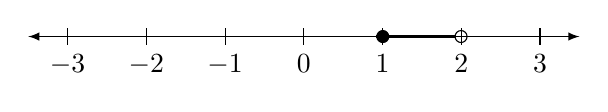
\begin{tikzpicture}
\draw[latex-latex] (-3.5,0) -- (3.5,0) ; %edit here for the axis
\foreach \x in  {-3,-2,-1,0,1,2,3} % edit here for the vertical lines
\draw[shift={(\x,0)},color=black] (0pt,3pt) -- (0pt,-3pt);
\foreach \x in {-3,-2,-1,0,1,2,3} % edit here for the numbers
\draw[shift={(\x,0)},color=black] (0pt,0pt) -- (0pt,-3pt) node[below] 
{$\x$};
\draw[*-o] (0.92,0) -- (2.08,0);
\draw[very thick] (0.92,0) -- (1.92,0);
\end{tikzpicture}

\begin{tcolorbox}
Let $Z$ be a standard-normal random variable... % TODO : get this section from coop or warner? 
\end{tcolorbox}

\subsection*{Sums of Independent Random Variables}

\nline
Let $f$ and $g$ be pdfs. The convolution integral is 

\begin{equation*}
(f \cdot g)(x) = \int_{- \int}^{\int} f(x-y) g(y) \enspace dy.
\end{equation*}

\nline
Let $x-y = \xi$. So, $d \xi = -dy$, and hence

\begin{align*}
(f \cdot g)(x) &= - \int_{\infty}^{- \infty} f(\xi) g(x- \xi) d \xi \\
&= \int_{- \infty}^{\infty} g(x- \xi) f(\xi) d \xi \\
&= (g \cdot f)(x) \\
\end{align*}

\nline
So, $\cdot$ is commutative. \textbf{Special Case}: Suppose that $f(x) = g(x) = 0$ for $x < 0$. Then, 

\begin{align*}
(f \cdot g)(x) &= \int_{- \infty}^{\infty} f(x-y) g(y) dy \\
&= \int_{0}^{\infty} f(x-y) g(y) dy \\
&= \int_{0}^{x} f(x-y) g(y) dy. \\
\end{align*}

\nline
Let $X$ and $Y$ be independent random variables with pdfs $f_X$ and $f_Y$ respectively. Let $Z = X + Y$ have pdf $f_Z$ with cdf $f_Z$. Let $f_X$ and $f_Y$ be the cdfs of $X$ and $Y$. 

\begin{align*}
F_Z(z) = \prob{Z \leq z} = \prob{X + Y \leq z} &= \int_{- \infty}^{\infty} \prob{X + Y \leq z \lvert Y = y} f_Y(y) dy \\
&= \int_{- \infty}^{\infty} \prob{X + y \leq z \lvert Y = y} f_Y(y) dy \\ 
&= \int_{- \infty}^{\infty} \prob{X \leq z - y \lvert Y = y} f_Y(y) dy \\
&= \int_{- \infty}^{\infty} \prob{X \leq z - y} f_Y(y) dy \\
&= \int_{- \infty}^{\infty} F_X(z-y) f_Y(y) dy.
\end{align*}

\noindent
So, $f_Z(z) = \frac{d}{dz} F_z(z) = \frac{d}{dz} \int_{- \infty}^{\infty} F_x (z-y) f_y (y) dy =  \int_{- \infty}^{\infty} F_x (z-y) f_y (y) dy = (f_x \cdot f_y)(z)$. In other words, $f_z(z)$ is equal to the convolution, $(f_x \cdot f_y)(z)$.

\begin{flushright}
\textbf{Date}: $11/9$
\end{flushright}

\subsection*{Sums of Independent Random Variables}
\nline
Recall that if $X$ and $Y$ are continuous and independent, with probability density function $f_x$ and $f_y$ then $Z = X + Y$ has probability density function 

\begin{equation*}
f_z(z) = (f_x \cdot f_y)(z) = \int_{- \infty}^{\infty} f_x (z-y) f_y(y) dy.
\end{equation*}

\noindent
The convolution is associative: $(f \cdot g) \cdot h = f \cdot (g \cdot h)$. We'll just write $f \cdot g \cdot h$ when grouping is not an issue. We may thus extend the convolution to any set $f_1, \ldots, f_n$ of probability density functions. So, if $X_1, \ldots, X_n$ are continuous, independent random variables with probability density functions $f_1, \ldots, f_n$ respectively, then $z = X_1 + \ldots + X_n$ has probability density function $f_z(z) = (f_1 \cdot \cdots \cdot f_n) (z)$. 

\begin{tcolorbox}
Let $X$ and $Y$ be normally distributed with mean $0$ and variance $1$. Let them be independent. Then $Z = X + Y$ is... ? Well,

\begin{center}
E($X + Y$) = E($X$) + E($Y$) = 0 \qquad V($X + Y$) = V($X$) + V($Y$) = 2
\end{center}

\begin{align*}
f_z(z) &= \int_{- \infty}^{\infty} \frac{1}{\sqrt{2 \pi}} e^{\frac{-(z-y)^2}{2}} \cdot \frac{1}{\sqrt{2 \pi}} e^{\frac{y^2}{2}} dy \\
&= \frac{1}{\sqrt{2 \pi}} \int_{- \infty}^{\infty} e^{- \frac{1}{2} \big [ (z-y)^2 + y^2 \big ]} dy \\
&= \frac{1}{\sqrt{2 \pi}} \int_{- \infty}^{\infty} e^{- \frac{1}{2} \big [ z^2 -2yz + 2y^2 \big ]} dy \\
&= \frac{e^{- \frac{1}{2} z^2 }}{\sqrt{2 \pi}} \int_{- \infty}^{\infty} e^{- (y^2  - yz)} dy \\
&= \frac{1}{\sqrt{2 \pi}} e^{- \frac{1}{2} z^2 } e^{\frac{1}{4} z^2 } \int_{- \infty}^{\infty} e^{- (y^2  - yz + \frac{1}{4}z^2 )} dy \\
&= \frac{1}{\sqrt{2 \pi}} e^{- \frac{1}{4} z^2 } \int_{- \infty}^{\infty} e^{- (y  - \frac{1}{2}z)^2} dy \\
\end{align*}

\begin{center}
\begin{tikzpicture}
% define normal distribution function 'normaltwo'
\def\normaltwo{\x,{4*1/exp(((\x-3)^2)/2)}}

% input y parameter
\def\y{3}

% this line calculates f(y)
\def\fy{4*1/exp(((\y-3)^2)/2)}

% Draw and label normal distribution function
\draw[color=blue,domain=0:6] plot (\normaltwo) node[right] {};

% Add dashed line dropping down from normal.
\draw[dashed] ({\y},{\fy}) -- ({\y},0) node[below] {$\frac{1}{2}z$};

% Optional: Add axes
\draw[->] (0,0) -- (6.2,0) node[right] {};
\draw[->] (0,0) -- (0,5) node[above] {};

\end{tikzpicture}
\end{center}

\noindent
Note that as you vary $z$, you do not change the value of the above integral.
\end{tcolorbox}

\nline
Let $T$ be exponentially distributed with parameter $\lambda > 0$. So, $T$ has probability density function 

\[ f(t) =  \begin{cases} 
      \lambda e^{- \lambda t} & \text{ for } t \geq 0, \\
      0 & \text{ for } t < 0.
      \end{cases} \]

\noindent
Thus, the $\expected{T} = \int_{- \infty}^{\infty} t f(t) dt = \frac{1}{\lambda}$, and $\variance{T} = \frac{1}{\lambda^2}$.

\nline
Let $T_1, \ldots, T_n$ be the service times for customers $1, \ldots, n$, respectively. Assume that the $T_j$ are iid exponentially distributed random variables, each wiit parameter $\lambda$. Thus, in this context, $\frac{1}{\lambda} = \expected{T}$ is the mean service time. Hence, $\lambda$ is the mean service rate (number of customers served per unit time). $\lambda$ is called the rate parameter. $S_n = T_1 + \cdots + T_n$ is time taken to serve $n$ customers. How is $S_n$ distributed? Let $g_n(t)$ be the probability distribution function of $S_n$. So, $g_1(t) = f(t)$,  $g_2(t) = (f \cdot f)(t)$, and $g_n(t) = (f \cdot \cdots \cdot f)(t)$. For $t \geq 0$, 

\begin{align*}
g_2(t) &= \int_{- \infty}^{\infty} f(t-s)f(s) ds \\
&= \int_{0}^{t} f(t-s)f(s) ds \\
&= \lambda^2 \int_{0}^{t} e^{- \lambda (t - s) } e^{- \lambda s} ds \\
&= \lambda^2 \int_{0}^{t} ds e^{- \lambda t} \\
&= \lambda^2 t e^{- \lambda t}. \\
\end{align*}

So, $T_1 + T_2 = S_2$ has probability distribution function 

\[ g_2(t) =  \begin{cases} 
      \lambda^2 t e^{- \lambda t} & \text{ for } t \geq 0, \\
      0 & \text{ otherwise}.
      \end{cases} \]

\noindent
The probability distribution function of $S_3 = T_1 + T_2 + T_3$ is (for $t \geq 0$)

\begin{align*}
g_3(t) = (f \cdot f \cdot f)(t) &= f \cdot (f \cdot f) (t) = (f \cdot g_2) (t) \\
&= \int_{0}^{t} \lambda e^{- \lambda (t-s)} \cdot \lambda^2 s ds = e^{- \lambda t} \int_{0}^{t} s ds \\
&= \frac{\lambda^3}{2} t^2 e^{- \lambda t}. \\
\end{align*}

\noindent
Therefore, $s_3$ has probability distribution function 

\[ g_3(t) =  \begin{cases} 
      \frac{\lambda^3}{2} t^2 e^{- \lambda t} & \text{ for } t \geq 0, \\
      0 & \text{ for } t < 0.
      \end{cases} \]
      
\noindent
By induction, $g_n(t)$, the probability distribution function of $s_n = T_1 + \cdots + T_n$ is 

\[ g_n(t) =  \begin{cases} 
      \frac{\lambda^n}{(n-1)!} t^{n-1} e^{- \lambda t} & \text{ for } t \geq 0, \\
      0 & \text{ for } t < 0.
      \end{cases} \]
      
\noindent
$g_n(t)$ is the probability distribution function of the Erlang distribution, with rate parameter $\lambda$ and shape parameter $n$. The gamma function is $\Gamma (x) = \int_{0}^{\infty} t^{x-1} e^{-t} dt$, defined for $x > 0$. For an integer $n > 0$, $\Gamma (n) = (n-1)!$. So, for $t \geq 0$, $g_n(t) = \frac{\lambda^n}{\Gamma(n)} t^{n-1} e^{- \lambda t}$. Let $\alpha > 0$. The probability distribution function for the gamma distribution, with rate parameter $\lambda$ and shape parameter $\alpha$ is 

\[ \begin{cases} 
      \frac{\lambda^{\alpha}}{\Gamma(\alpha)} t^{\alpha -1} e^{- \lambda t} & \text{ for } t \geq 0, \\
      0 & \text{ for } t < 0.
      \end{cases} \]
      
\begin{flushright}
\textbf{Date}: $11/16$
\end{flushright}

\noindent
\[ g_1(t) = \begin{cases} 
      \lambda e^{- \lambda t} & \text{ for } t \geq 0, \\
      0 & \text{ for } t < 0.
      \end{cases} \]

\noindent
Then, we have $g_2(t) = (g_1 \cdot g_1)(t), \ldots, g_n (t) = (g_1 \cdots g_1)(t) = (g_1 \cdot g_{n-1})(t)$. This generalizes to

\[ g_n(t) = \begin{cases} 
      \frac{\lambda^{n}}{\Gamma(n)} t^{n -1} e^{- \lambda t} & \text{ for } t \geq 0, \\
      0 & \text{ for } t < 0.
      \end{cases} \]
      
\noindent
For $\beta$ not necessarily an integer, we define the gamma density with rate parameter $\lambda > 0$ and shape $\beta > 0$, 

\[ g_n(t) = \begin{cases} 
      \frac{\lambda^{\beta}}{\Gamma(\beta)} t^{\beta -1} e^{- \lambda t} & \text{ for } t \geq 0, \\
      0 & \text{ for } t < 0.
      \end{cases} \]
      
\noindent
Let $T_1, \ldots, T_n$ be service times for customers in a queuing system. we follow the simplest model ($m$/$m$/$1$) of queues. The $T_k$ is identically and independently exponentially distributed random variables (iid's). Let $\lambda$ be their common rate parameter. Then, $\expected{T_k} = \frac{1}{\lambda}$ and $\variance{T_k} = \frac{1}{\lambda^2}$ for $k = 1, \ldots, n$. The time required to serve all $n$ customers is $S_n = T_1 + \cdots + T_n$. Therefore, $S_n$ is Erlang/gamma distributed - its probability distribution function is $g_n(t)$.

Hence, since $T_k$ is iid, $\expected{S_n} = n \expected{T_1} = \frac{n}{\lambda}$ and $\variance{S_n} = n \variance{T_1} = \frac{n}{\lambda^2}$. 

\begin{tcolorbox}
\noindent
Consider a small caf\'e with one barista and iid exponential service times with rate parameter $\lambda = .4/\text{min}$. Let $A_n$ be the event that, upon your arrival, there are $n$ customers in line ahead of you. Let $T$ be your unconditional total time in the system. Thus, your total (waiting + service) in the queuing system is 

\begin{equation*}
S_{n+1} = T_1 + \cdots + T_n + T_{n+1}
\end{equation*}

\noindent
where $T_1, \ldots, T_n$ are the service times of those ahead of you, and $T_{n+1}$ your service time$^*$. Hence, your time $S_{n+1}$, given $A_n$ is gamma distributed with rate parameter $\lambda = .4/\text{min}$ and shape parameter $n+1$. So, 

\begin{equation*}
\condprob{T > t}{A_n} = \prob{S_{n+1} > t} = \int_{t}^{\infty} g_{n+1}(s) ds = \frac{.4^{n+1}}{n!} \int_{t}^{\infty} s^n e^{-.4s} ds.
\end{equation*}

\noindent
In $R$, this can be written as 

\begin{equation*}
\text{pgamma}(t, n+1 .4, lower.tail=FALSE) = \text{pgamma}(t, n+1 .4, lower=F) = 1 - \text{pgamma}(t, n+1 .4) .
\end{equation*}

For example, 

\begin{equation*}
\condprob{T > 10}{A_3} = \prob{S_{4} > 10} =   \text{pgamma}(t0, 4 .4, lower.tail=FALSE) = 0.43347.
\end{equation*}

\vspace*{.5cm}
$^*$ Conditional time in the system, given $A_n$.
\end{tcolorbox}

\noindent
What is the unconditional distribution of $T$?

\noindent
For queuing in equilibrium, the probability that the system state (number of customers in line at the caf\'e) is $(1-\rho)\rho^n$ where $\rho = \frac{\mu}{\lambda}$ where $\mu$ is the mean arrival wait,

\begin{align*}
\prob{T > t} &= \sum_{n = 0}^{\infty} \condprob{T > t}{A_n} \prob{A_n} \qquad (\text{Law of Total Probability}) \\
&= \sum_{n = 0}^{\infty} \prob{S_{n+1} > t} (1- \rho) \rho^n \\
&= \sum_{n = 0}^{\infty} \frac{\lambda^{n+1}}{n!} \int_{t}^{\infty} s^n e^{- \lambda s} ds (1- \rho) \rho^n \\
&= (1- \rho) \lambda \int_{t}^{\infty} \sum_{n = 0}^{\infty} \frac{(\lambda \rho s)^{n}}{n!} e^{- \lambda s} ds \\
&= (1- \rho) \lambda \int_{t}^{\infty}  e^{\lambda \rho s} e^{- \lambda s} ds \\
&= (1- \rho) \lambda \int_{t}^{\infty} e^{- \lambda (1-\rho) s} ds. \\
&= (1- \rho) \lambda \Bigg [ \frac{e^{- \lambda (1-\rho) s}}{- \lambda (1 - \rho)} \Bigg ]_{s=t}^{s=\infty}. \\
\end{align*}
%&= (1- \rho) \lambda \frac{e^{- \lambda (1-\rho) t}}{\lambda (1 - \rho)} \\
%&= e^{- \lambda (1-\rho) t}} \\

\noindent
Thus, $T$ is exponentially distributed with parameter $\lambda (1 - \rho)$. So, your expected (unconditional) total time in the system is $\expected{T} = \frac{1}{\lambda (1 - \rho)}$.

\subsubsection*{Rayleigh Distribution}
Let $X$ and $Y$ be independent, standard normal variables. So, 

\begin{equation*}
f_X(x) = f_Y(y) = \frac{1}{\sqrt{2 \pi}} e^{- \frac{x^2}{2}}. 
\end{equation*}

\noindent
Then, how is $X^2$ distributed? Well, $\prob{X^2 \leq r} = F_{X^2} (r) = \prob{- \sqrt{r} \leq X \leq \sqrt{r}} = \frac{1}{\sqrt{2 \pi}} \int_{- \sqrt{r}}^{\sqrt{r}} e^{- \frac{x^2}{2}} dx = \frac{2}{\sqrt{2 \pi}} \int_{0}^{\sqrt{r}} e^{- \frac{x^2}{2}}$. Hence, the probability distribution function of $X^2$

\begin{align*}
f_{X^2}(r) = F_{X^2}^{'} (r) &= \frac{2}{\sqrt{2 \pi}} e^{- \frac{r}{2}} \cdot \frac{1}{2 \sqrt{r}} \\
&= \frac{1}{\sqrt{2 \pi r}} e^{- \frac{r}{2}}, 
\end{align*}

\noindent
for $r > 0$.

\begin{tcolorbox}
\begin{align*}
\Gamma(\frac{1}{2}) = \int_{0}^{\infty} t^{\frac{1}{2} - 1} e^{-t} dt &= \int_{0}^{\infty} \frac{e^{-t}}{\sqrt{t}} dt \\
&= \int_{0}^{\infty} \frac{e^{-u^2}}{u} 2u \enspace du \\
&= 2 \int_{0}^{\infty} e^{-u^2} du \\
&= 2 \int_{- \infty}^{\infty} e^{-u^2} du \\
&= \sqrt{\pi}.
\end{align*}

\noindent
The gamma density with rate parameter $\lambda = \frac{1}{2}$ and shape parameter $\beta = \frac{1}{2}$ is

\begin{equation*}
g(r) = \frac{(\frac{1}{2})^{\frac{1}{2}} r^{\frac{1}{2} - 1}}{\Gamma(\frac{1}{2})} e^{- \frac{1}{2} r}
= \frac{1}{\sqrt{2 \pi r}} e^{- \frac{1}{2} r},
\end{equation*}

for $r > 0$.

Thus, $X^2$ and $Y^2$ are gamma distributed with $\lambda = \frac{1}{2}$ and $\beta = \frac{1}{2}$.
\end{tcolorbox}

\begin{flushright}
\textbf{Date:} $11/28$
\end{flushright}

\subsection*{7.1 The (weak) Law of Large Numbers}

\noindent
Let $\big \{ x_k \big \}_{k=1}^{\infty}$ be i.i.d. random variables, with means $\expected{x_k} = \mu$ and variance $\variance{x_k} = \sigma^2$, $k = 1, 2, 3, \ldots$ where $\mu$ and $\sigma^2$ are finite. Let $S_n = X_1 + \ldots + X_n$. How is $\frac{S_n}{n}$ distributed for ``large'' $n$? Consider the degenerate \textit{probability mass function} ,

\[ p(x) = \begin{cases} 
      1 & \text{ if } x = \mu, \\
      0 & \text{ otherwise.}.
      \end{cases} \]

\noindent
In some sense, it should be that $\frac{S_n}{n}$ (approximately) has \textit{probability mass function} $p$ for $n$ ``large''. This statement is the assertion of the \textit{Weak Law of Large Numbers}, 

\begin{center}
For $\epsilon > 0$, $\lim_{n \leftarrow \infty} P(\lvert \frac{S_n}{n} - \mu \rvert < \epsilon) = 1$.
\end{center}

\begin{tcolorbox}
\noindent
\textbf{Proof} The expected value can be calculated as follows, 

\begin{equation*}
\expected{\frac{S_n}{n}} = \frac{1}{n} \expected{S_n} = \frac{1}{n} n \mu = \mu.
\end{equation*}

\noindent
The variance can be calculated as follows, 

\begin{equation*}
\variance{\frac{S_n}{n}} = \frac{1}{n^2} \variance{S_n} = \frac{1}{n^2} n V(X_1) = \frac{1}{n} \sigma^2.
\end{equation*}

\noindent
Then, 

\begin{equation*}
P(\lvert \frac{S_n}{n} - \mu \rvert < \epsilon) + P(\lvert \frac{S_n}{n} - \mu \rvert \geq \epsilon) = 1.
\end{equation*}

\noindent
By Chebysev, $P(\lvert \frac{S_n}{n} - \mu \rvert \geq \epsilon) \leq \frac{\sigma^2}{n \epsilon^2} \rightarrow 0 \text{ as } n \rightarrow \infty$. By plugging this into the equation directly above, letting $n \rightarrow \infty$, 

\begin{equation*}
\lim_{n \rightarrow \infty} P(\lvert \frac{S_n}{n} - \mu \rvert < \epsilon) = 1.
\end{equation*}
\end{tcolorbox}

\vspace*{.5cm}

\begin{tcolorbox}
\textbf{Example} Coin flips: Let $\big \{ x_k \big \}_{k=1}^{\infty}$ be a sequence of i.i.d. Bernoulli random variables with ranges $\{ 0, 1\}$ and common \textit{probability mass function} $p(0)=p(1) = .5$. Think of $X_k$ as the ``head-counting'' variable for a sequence of fair coin flips. So, 

\[ X_k = \begin{cases} 
      0 & \text{ if ``Tail'' on flip } k, \\
      1 & \text{ if ``Head'' on flip } k.
      \end{cases} \]
  
 \noindent
So, $S_n = \sum_{k = 1}^{n} X_k$ is the number of heads observed in $n$ flips. We know that $\expected{X_k} = .5$ and that $\variance{X_k} = .25$. So, by the \textit{Weak Law of Large Numbers}, for any $\epsilon > 0$, 
 
 \begin{equation*}
 \lim_{n \rightarrow \infty} P(\lvert \frac{S_n}{n} - .5 \rvert < \epsilon) = 1.
 \end{equation*}
\end{tcolorbox}

\noindent
Since $\variance{\frac{S_n}{n}} \rightarrow 0$ as $n \rightarrow \infty$, the support of the probability mass function (or probability density function) of $\frac{S_n}{n}$ is collapsing to the single point $\mu$. Consider $\frac{S_n}{\sqrt{n}}$. Then, $\variance{\frac{S_n}{\sqrt{n}}} = \frac{1}{n} \variance{S_n} = \frac{1}{n} n \variance{X_1} = \sigma^2$. Since $\variance{\frac{S_n}{\sqrt{n}}}$ does not go to $0$, can we say anything about the asymptotic distribution of $\frac{S_n}{\sqrt{n}}$? Note that $\expected{\frac{S_n}{\sqrt{n}}} = \sqrt{n} \mu \rightarrow \infty$ as $n \rightarrow \infty$. Hence in considering the asymptotic behavior of $\frac{S_n}{\sqrt{n}}$, we have to make one more adjustment. We ``center'' the $X_k$ by subtracting their means $\mu$. While we're at it, we may as well normalize variances to $1$. In summary, we consider the ``standardized'' random variables

\begin{equation*}
X_{k}^{*} = \frac{X_k - \mu}{\sigma}.
\end{equation*}

\noindent
The expected value is then $\expected{X_{k}^{*}} = \frac{1}{\sigma} \expected{X_k - \mu} = 0$ and the variance is $\variance{X_{k}^{*}} = \variance{\frac{X_{k} - \mu}{\sigma}} = \frac{1}{\sigma^2} \variance{X_k - \mu} = 1$. Let $S_{n}^{*} = X_{1}^{*} + \ldots + X_{n}^{*}$. 

\vspace*{.5cm}
\noindent
\textbf{Question}: How does $\frac{S_{n}^{*}}{\sqrt{n}}$ behave as $n \rightarrow \infty$? Bear in mind, $\expected{\frac{S_{n}^{*}}{\sqrt{n}}} = 0$ and $\variance{\frac{S_{n}^{*}}{\sqrt{n}}} = \frac{1}{n} n = 1$.

\vspace*{.5cm}
\noindent
Well, let the $X_k$ be i.i.d. exponentials with $\lambda = 2$. Using $R$, we generate $1000$ samples values and plotted the histogram. Numerical evidence suggests that for $n$ large, $\frac{S_{n}^{*}}{\sqrt{n}} \sim N(0,1)$, approximately.

% TODO: insert the picture of the histogram and the r code

\vspace*{.5cm}
\noindent
We prove (sort of) that this is indeed the case, by means of moment generating functions. The moment generating function (MGF) $g_x(t)$ of a random variable $X$ is $g_X(t) = \expected{e^{tX}}$. 

\begin{tcolorbox}
\textbf{Example} Let $X$ be Poisson distributed, with mean $\lambda$. Then, 

\begin{equation*}
g_X(t) = \expected{e^{tX}} = \sum_{n=0}^{\infty} e^{tn} \frac{\lambda^n}{n!} e^{- \lambda} = e^{- \lambda} \sum_{n=0}^{\infty} \frac{(e^{t}\lambda)^n}{n!} = e^{- \lambda} e^{\lambda e^{t}} = e^{\lambda (e^{t} - 1)}.
\end{equation*}
\end{tcolorbox}

\begin{tcolorbox}
\textbf{Example} Let $X$ be Gaussian distributed, with mean $0$ and variance $1$. Then, 

\begin{align*}
g_X(t) &= \frac{1}{\sqrt{2 \pi}} \int_{- \infty}^{\infty} e^{tn} e^{- \frac{x^2}{2}} dx \\
&=  \frac{1}{\sqrt{2 \pi}} \int_{- \infty}^{\infty} e^{- \frac{1}{2}(x^2 - 2tx + t^2)} dx \cdot e^{\frac{1}{2} t^2} \\
&= \frac{1}{\sqrt{2 \pi}} \int_{- \infty}^{\infty} e^{- \frac{1}{2}(x-t)} dx \cdot e^{\frac{1}{2} t^2} \\
&= \frac{\sqrt{2 \pi}}{\sqrt{2 \pi}} e^{\frac{1}{2} t^2} \text{, using Liouville's formula} \\
&= e^{\frac{1}{2} t^2}
\end{align*}
\end{tcolorbox}

\noindent
Skipping some technical details,

\begin{center}
$X$ and $Y$ have the same distribution $\leftrightarrow$ $g_X(t) = g_Y(t)$. 
\end{center}

\noindent
The \textbf{Central Limit Theorem} (CLT) asserts that $\frac{S_{n}^{*}}{\sqrt{n}}$ is asymptotically standard-normal as $n \rightarrow \infty$. We will prove this by showing that 

\begin{equation*}
g_{\frac{S_{n}^{*}}{\sqrt{n}}}(t) \longrightarrow e^{\frac{1}{2} t^2} \text{ as } n \rightarrow \infty. 
\end{equation*}

\noindent
We will need these properties:

\begin{itemize}
\item Let $X$ and $Y$ be independent with MGF's $g_X$ and $g_Y$, respectively. Then, $g_{X+Y}(t) = g_X(t) g_Y(t)$.

\textbf{Proof}: $g_{X+Y}(t) = \expected{ e^{t (X+Y)}} = \expected{ e^{t X} e^{t Y}} = \expected{ e^{t X}} \cdot \expected{ e^{t Y}} = g_X(t) g_Y(t)$.

\item Let $X$ have MGF $g_X(t)$. Then, for any constant $c$, $g_{cX}(t) = g_X(ct)$.

\textbf{Proof}: $g_{cX}(t) = \expected{ e^{t (cX)}} = \expected{ e^{(ct) X}} = g_X(ct)$.

\item Let $g(t)$ be the MGF of $X_{k}^{*}$. The $X_{k}^{*}$ are i.i.d. and hence 

\begin{equation*}
g_{\frac{S_{n}^{*}}{\sqrt{n}}}(t) = g_n(t) = g_{\frac{X_{1}^{*} + \cdots + X_{n}^{*}}{\sqrt{n}}} (t) = g_{X_{1}^{*} + \cdots + X_{n}^{*}}(\frac{t}{\sqrt{n}}) = g \big ( \frac{t}{\sqrt{n}} \big )^n
\end{equation*} 
\end{itemize}

% TODO: get make up dayz...

\begin{flushright}
\textbf{Date:} $12/5$
\end{flushright}

\noindent
\textbf{CLT} Example: Roll a fair die $500$ times. So, $n=500$. Let $S_{500}$ be the number of $1$'s. Use the CLT to estimate $\prob{80 \leq S_{500} \leq 110}$. Then, let

\[ X_k = \begin{cases} 
      1 & \text{ if ``$1$'' on roll } k, \\
      0 & \text{ otherwise on roll } k
      \end{cases} \]
      
\noindent
for $k = 1, \ldots, 500$. Assume that $X_k$ are independent. Thus, they are i.i.d. with means $\mu = \expected{X_k} = \frac{1}{6}$ and variances $\variance{X_k} = \frac{1}{6} \cdot \frac{5}{6} = \frac{5}{36}$. Therefore, $D(X_k) = \sigma = \frac{\sqrt{5}}{6}$. So, $n=500$, $\mu = \frac{1}{6}$, $\sigma = \frac{\sqrt{5}}{6}$, and $S_{500} = \sum_{k=1}^{500} X_k$. So,

\begin{align*}
\prob{80 \leq S_{500} \leq 110} &= \prob{\frac{80-n \mu}{\sqrt{n} \sigma} \leq \frac{S_n}{\sqrt{n}} \leq \frac{110-n \mu}{\sqrt{n} \sigma}} \\
&= \prob{-.894 \leq \frac{S_n}{\sqrt{n}} \leq .7155} \sim \Phi(7.155) - \Phi(-.894) \\
&= \text{pnorm}(7.155,0,1) - \text{pnorm}(-.894,0,1) = .8144. 
\end{align*}

\noindent
Note that $S_{500}$ is actually binomial with parameters $$ and $$. So, in $R$, $\prob{80 \leq S_{500} \leq 110} = \text{pnorm}(10,500,1/6) - \text{pnorm}(80,500,1/6) = .628$.

\begin{tcolorbox}
\textbf{Example} The ``lifespan'' of a certain type of industrial drill bit is the number of hours of continuous use before the bit must be discarded. For one type of drillbit, the lifespan is exponentially distributed with mean $\frac{1}{\lambda} = 5.2$ hour - $\lambda$ is the rate parameter. Let $T_1 + \cdots + T_{100}$ be the lifespan of $100$ such bits. We assume them to be i.i.d. exponentials. Let $S_{100} = T_1 + \cdots + T_{100}$. Use the CLT to estimate $\prob{550 \leq S_{100}}$. Observe that $\expected{S_{100}} = 520$. Here, $n = 100$, $\mu = \expected{T_k} = 5.2$, and $\variance{T_k} = 5.2^2$, so that $\sigma = 5.2$ also. Hence, $\prob{550 \leq S_{100}} = \prob{\frac{550-100 \cdot 5.2}{10 \cdot 5.2} \leq \frac{S_{100}}{10}}$. The distribution is approximately standard normal for ``large'' $n$.

\vspace*{.5cm}
\noindent
We see that $\prob{\frac{550-100 \cdot 5.2}{10 \cdot 5.2} \leq \frac{S_{100}}{10}} = \prob{\frac{30}{52} \leq \frac{S_{100}}{10}} \sim 1 - \Phi(\frac{15}{26}) = .282$. So, $S_{100}$ is actually gamma (or Erlang) distributed with shape parameter $n=100$ and rate parameter $\lambda = \frac{1}{5.2}$. So, $\prob{550 \leq S_{100}} = \frac{\lambda^100}{99!} \int_{550}^{\infty} t^{99} e^{- \lambda t} dt = 1 - \text{pgamma}(550, 100, \lambda)$. We subtract from $1$ here, but we can also specify that \textit{tail=false} in the \textit{pgamma} function in $R$.
\end{tcolorbox}


\subparagraph*{Brownian Motion} Consider a ``Brownian particle'' moving random but continuously on the x-axis, with initial position $x = 0$. Let $t > 0$ be fixed. Let $B_t$ be the random variable representing the position of the particle on the $x$-axis at time $t$. How is $B_t$ distributed? We'll start with a ``random walk'' on $[0,t]$. Divide $[0,t]$ into $n$ sub-intervals, each of duration $\triangle t = \frac{t}{n}$. Let $t_0 = 0$, $t_1 = \triangle t$, $t_2 = 2 \triangle t$, $\ldots$, $t_n = n \triangle t$ be the endpoints of the sub-intervals. In each sub-interval, the particle moves a distance $\triangle x$, either to the left or to the right. Define the variables $\xi_1, \ldots, \xi_n$ by

\[ \xi_k = \begin{cases} 
      1 & \text{ if particle moves to the right in subinterval k}, \\
      -1 & \text{  if particle moves to the left in subinterval k}.
      \end{cases} \]

\noindent
Let $x_k = \xi_k \triangle x$. So, the position of the particle at time $t$ is $x_1 + \ldots + x_n = S_n$. Assume that the $xi_k$ are i.i.d. with $\prob{\xi_k = 1} = \prob{\xi_k = -1} = .5$. The random walk is ``symmetric''. With additional stipulations, we take $\prob{a \leq B_t \leq b} = \lim_{n \rightarrow \infty} \prob{a \leq S_n \leq b}$.

\begin{equation*}
\prob{a \leq S_n \leq b} = \prob{a \leq (\xi_1 + \cdots + \xi_n) \triangle x \leq b} = \prob{\frac{a}{\triangle x} \leq \xi_1 + \cdots + \xi_n \leq \frac{b}{\triangle x}}.
\end{equation*}

\noindent
Observe that the $\xi_k$ are i.i.d. with mean $\expected{\xi_k} = 0 = \mu$ and variances $\variance{\xi_k} = 1 \text{ } (\sigma = 1)$. Thus, $\xi_1 + \cdots + \xi_n = S_n$. So, the equation above becomes 

\begin{equation*}
\prob{a \leq S_n \leq b} = \prob{\frac{a}{\triangle x} \leq S_n \leq \frac{b}{\triangle x}} = \prob{\frac{a}{\sqrt{n} \triangle x} \leq \frac{S_n}{\sqrt{n}} \leq \frac{b}{\sqrt{n} \triangle x}}.
\end{equation*}

\vspace*{.5cm}
\noindent
We know that $n \triangle = t$. The diffusion coefficient $D = \frac{\triangle x^2}{2 \triangle t}$. Probabilists usually set $D = \frac{1}{2}$, so that $\frac{\triangle x^2}{\triangle t} = 1$, or $\frac{\triangle x}{\sqrt{ \triangle t}} = 1$. So, the above equation becomes 

\begin{equation*}
\prob{a \leq S_n \leq b} = \prob{\frac{a}{\sqrt{n} \triangle x} \leq \frac{S_n}{\sqrt{n}} \leq \frac{b}{\sqrt{n} \triangle x}} = \prob{\frac{a}{\sqrt{n \triangle x} \frac{\triangle x}{\sqrt{\triangle t}}} \leq \frac{S_n}{\sqrt{n}} \leq \frac{b}{\sqrt{n \triangle x} \frac{\triangle x}{\sqrt{\triangle t}}}} = \prob{\frac{a}{\sqrt{t}} \leq \frac{S_n}{\sqrt{n}} \leq \frac{b}{\sqrt{t}}}. 
\end{equation*}

\noindent
Therefore, 

\begin{align*}
\prob{a \leq S_n \leq b} &= \lim_{n \rightarrow \infty} \prob{a \leq S_n \leq b} \\
&= \lim_{n \rightarrow \infty} \prob{\frac{a}{\sqrt{t}} \leq S_n \leq \frac{b}{\sqrt{t}} } \\
&= \frac{1}{\sqrt{2 \pi}} \int_{\frac{a}{\sqrt{t}}}^{\frac{b}{\sqrt{t}}} e^{- \frac{z^2}{2}} dz\\
&= \frac{1}{\sqrt{2 \pi}} \int_{a}^{b} e^{- \frac{u^2}{2t}} \frac{du}{\sqrt{dt}}\\
&= \frac{1}{\sqrt{2 \pi t}} \int_{a}^{b} e^{- \frac{u^2}{2t}} du
\end{align*}

\noindent
Hence, $B_t$ is Gaussian with mean $0$ and variance $t$.

\vspace*{.5cm}
\noindent
A \textbf{stochastic process} is a collection of random variables. We usually study stochastic processes of the form $\big \{ X_n \big \}_{n=0}^{\infty} = \big \{ X_0, X_1, \ldots \big \}$ or $\big \{ X_t \big \}_{t \geq 0}$. $n$ and $t$ usually represent discrete and continuous time. Thus, $X_3$ represents the ``state'' of the process at time $n=3$ or $t=3$. We showed that the position $B_t$ of the Brownian particle was a Gaussian variable with mean $0$ and variance $t$. $\big \{ B_t \big \}_{t \geq 0}$ is a stochastic process with $\prob{B_0 = 0} = 1$. Brownian motion is seen as important in statistical mechanics, quantum mechanics, stochastic differential equations, and finance.

\vspace*{.5cm}
\noindent
% http://galton.uchicago.edu/~lalley/Courses/313/WienerProcess.pdf
We assume that Brownian Motion (the Wiener Process) has \textbf{independent} and \textbf{stationary} increments. Clearly, $B_s$ and $B_t$ are not independent. But, it is reasonable to assume that $B_t - B_s$ and $B_s - B_r$ are independent. This is the assumption of independent increments. For any times $t_1, \ldots, t_n$, $B_{t_1 + s} - B_{t_1}, ldots, B_{t_n + s} - B_{t_n}$ have the same distribution. What is that distribution? Well, $B_{t_k + s} - B_{t_k}$ has the same distribution as $B_{0  + s} - B_{0} = B_{s}$, which is Gaussian with mean $0$ and variance $s$. Thus, for any $t$, the increment $B_{t+s} - B_t$ is Gaussian, mean $0$, variance $s$. 

\begin{tcolorbox}
Let $t_0 = 0$, $x_0 = 0$, and then $0 < t_1 < t_2$. Let $I_1$ and $I_2$ be intervals on the $x$-axis. What is $\prob{B_{t_1} \in I_1, B_{t_2} \in I_2}$?

\vspace*{.5cm}
First, the particle must reach a point $x_1 \in I_1$ at time $t_1$. From $x_1$, it must reach a point $x_2 \in I_2$, in time period of length $t_2 - t_1$. So, by independent and stationary increments, 

% if you have a bag of all the functions, what is the probability that you pull out a continuous functions taht are not differentiable anywhere?
\begin{equation*}
\prob{B_{t_1} \in I_1, B_{t_2} \in I_2} = \frac{1}{\sqrt{2 \pi (t_1 - t_0)}} \frac{1}{\sqrt{2 \pi (t_2 - t_1)}} \int_{I_2} \int_{I_1} e^{\frac{-(x_1-x_0)^2}{2t_1}} e^{\frac{-(x_2-x_1)^2}{2(t_2 - t_1)}} dx_1 dx_2
\end{equation*}
\end{tcolorbox}

\noindent
We also know there are different types of Brownian motion,

\begin{itemize}
% big in financial analysis
\item Geometric Brownian Motion: $X_t = A e^{B_t}$
\item Integrated Brownian Motion: $X_t = \int_{0}^{t} B_s ds$
\item Brownian Bridge: $X_t = B_t - \frac{t}{T} B_T$
\end{itemize}

% TODO: type up poisson process notes
How many punctual events occur in the period $(0, t]$? Let the number be $N_t$. $\prob{N_0} = 0$. $\{ N_t \}_{t \geq 0}$ is called the Poisson process. How is $N_t$ distributed? Divide $(0, t]$ into $n$ sub-intervals, each of length $\Delta \frac{t}{n}$. Assume that in each sub-interval, the probability $\prob{N_t = k}$? Let $\lambda$ be the mean occurrence rate per unit time. Then, $\prob{N_t = k} = \frac{(\lambda t)^k}{k!} e^{- \lambda t}$. Customers arrive at a cafe according to a Poisson process with rate parameter $\lambda = .25$/min. What is the probability that between $5$ and $8$ customers arrive during the period 12:00 and 12:32? 

% \lambda = .25, t = 32
\begin{align*}
\prob{5 \leq N_{32} \leq 8} &= \sum_{k=5}^{8} \frac{(\lambda t)^k}{k!} e^{- \lambda t} \\
&= \sum_{k=5}^{8} \frac{(8^k}{k!} e^{- 8} \\
&= .493
\end{align*}

% pg 338: 1,2,3,5,10,12

\begin{equation*}
\int_0^{\infty} f(x) dx.
\end{equation*}
\end{document} 